\documentclass[xcolor=pdftex,dvipsnames,table,mathserif,aspectratio=169]{beamer}
\usetheme{metropolis}
%\usetheme{Darmstadt}
%\usepackage{times}
%\usefonttheme{structurebold}

\usepackage[english]{babel}
%\usepackage[table]{xcolor}
\usepackage{pgf,pgfarrows,pgfnodes,pgfautomata,pgfheaps}
\usepackage{amsmath,amssymb,setspace,centernot}
\usepackage[latin1]{inputenc}
\usepackage[T1]{fontenc}
\usepackage{relsize}
\usepackage{pdfpages}
\usepackage[absolute,overlay]{textpos} 



\DeclareMathSizes{10}{10}{6}{6} 


\title [Dynamic Demand I]{Learning Models and Experience Goods}
\author{C.Conlon}
\institute{Grad IO }
\date{Fall 2019}
\setbeamerfont{equation}{size=\tiny}
\begin{document}

\begin{frame}
\titlepage
\end{frame}



\section*{Introduction}
%\begin{frame}{State Dependence}
%Think about a static model like BLP
%\begin{eqnarray*}
%u_{ijt} = \beta_i x_{jt} - \alpha_i p_{jt} + \xi_{jt} + \epsilon_{ijt}
%\end{eqnarray*}
%\begin{itemize}
%\item Suppose I have panel data on consumer $i$'s purchases and I observe that the consumer chooses different brands over time
%\item Why do you switch brands? 
%\begin{enumerate}
%\item New $\epsilon \rightarrow$ not helpful!
%\item Price responses $\rightarrow$ may wrongly attribute all effects to price.
%\item $\xi_{jt}$ not correlated across individuals but may include things like advertising, etc.
%\end{enumerate}
%\item Challenge is explaining both \alert{persistence} and \alert{switching} behavior.
%\end{itemize}
%\end{frame} 



\begin{frame}{Uncertainty and Learning}
\begin{itemize}
\item We have already looked at models with forward looking consumers
\item Consumers faced uncertainty about the price, but understood the characteristics and the utility received from the good up to the IID $\epsilon$.
\item In many cases, consumers do not fully understand their preferences over goods until they sample the goods themselves.
\item Changes to brands, introduction of new brands, price cuts, coupons, or advertising may induce consumers to resample.
\item We would like to incorporate \alert{persistence} in brand choice but also \alert{experiential learning}
\end{itemize}
\end{frame} 


 
\begin{frame}{Uncertainty and Learning}
We examine three papers dealing with uncertainty and learning:
\begin{itemize}
\item Ackerberg (2001) looks at whether advertising lets consumers learn about new brands and distinguishes between informative and prestige effects
\item Erdem and Keane (1996) extends models of brand choice to allow for Bayesian learning about experience goods
\item Crawford and Shum (2005) look at how doctor's learn about patient's types as well as drug efficacy in a model of experiential learning.
\item Dickstein (2018) studies adherence to anti-depressants and learning with Gittin's index.
\end{itemize}
\end{frame}

\section*{Ackerberg}
\begin{frame}{Ackerberg 2001: Advertising and Yoplait 150}
\begin{itemize}
\item \textbf{Informative} about product existence and search characteristics. Stigler (1961), Butters (1977), Grossman Shapiro (1984) should not affect behavior of experienced users.
\item \textbf{Signalling} Nelson (1974), Kihlstrom and Riordan (1984), Milgrom and Roberts (1986).
\begin{enumerate}
\item If consumer perfectly learns about brand's experience characteristics after consumption $\rightarrow$ does not affect behavior of experienced users
\item If consumer continues to learn about  experience characteristics after consumption $\rightarrow$ should be decreasing in number of consumption experiences.
\end{enumerate}
\item \textbf{Prestige} Becker or Becker and Murphy (1993) does not depend on whether or not consumers have experienced the good but enters utility.
\end{itemize}
\end{frame}

\begin{frame}{Ackerberg 2001: Advertising and Yoplait 150}
\begin{itemize}
\item Ackerberg exploits panel data following advertising and grocery purchases over time.
\item Hypothesis is that \alert{informative} advertising has a larger effect on consumers with no brand experience.
\item \alert{Prestige} affects all consumers equally independent of experience.
\item Looks at a new product introduction to get around \alert{initial conditions problem}
\end{itemize}
\end{frame}

\begin{frame}{Ackerberg 2001: Data}
\begin{itemize}
\item AC Neilsen \textit{Scanner Data} matched upw ith TV meters
\item 1986-1989 covers 2000 households and 80\% of area drugstores and supermarkets.
\item Two cities: Sioux Falls, SD \alert{(SF)} and Springfield, MO \alert{(SP)}
\item He chooses yogurt because it is not easily storable (Hendel Nevo 2007).
\item Introduction of \alert{Yoplait 150} by the \#2 manufacturer
\item Heavily advertised, first low-fat, low-calorie yogurt by Yoplait!
\end{itemize}
\end{frame}

\begin{frame}{Table 1: Descriptive Statistics}
\begin{figure}[htbp]
\begin{center}
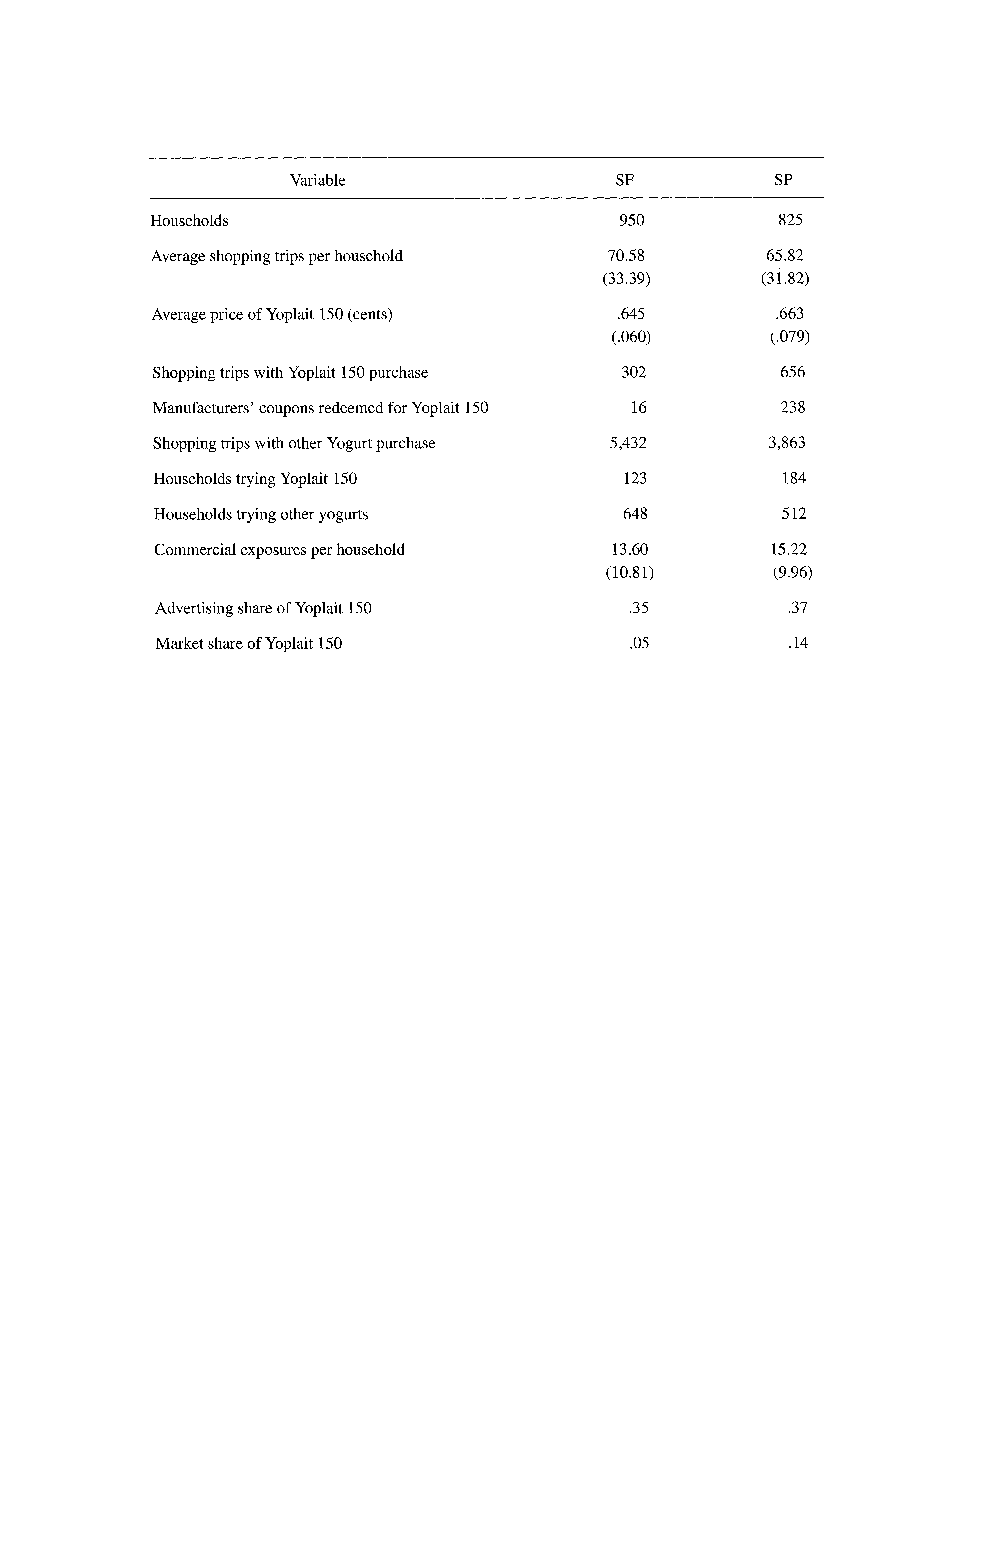
\includegraphics[width=8.5cm]{resources/acker1.pdf}
\label{default}
\end{center}
\end{figure}
\end{frame}

\begin{frame}{Table 2: Descriptive Correlations}
\begin{figure}[htbp]
\begin{center}
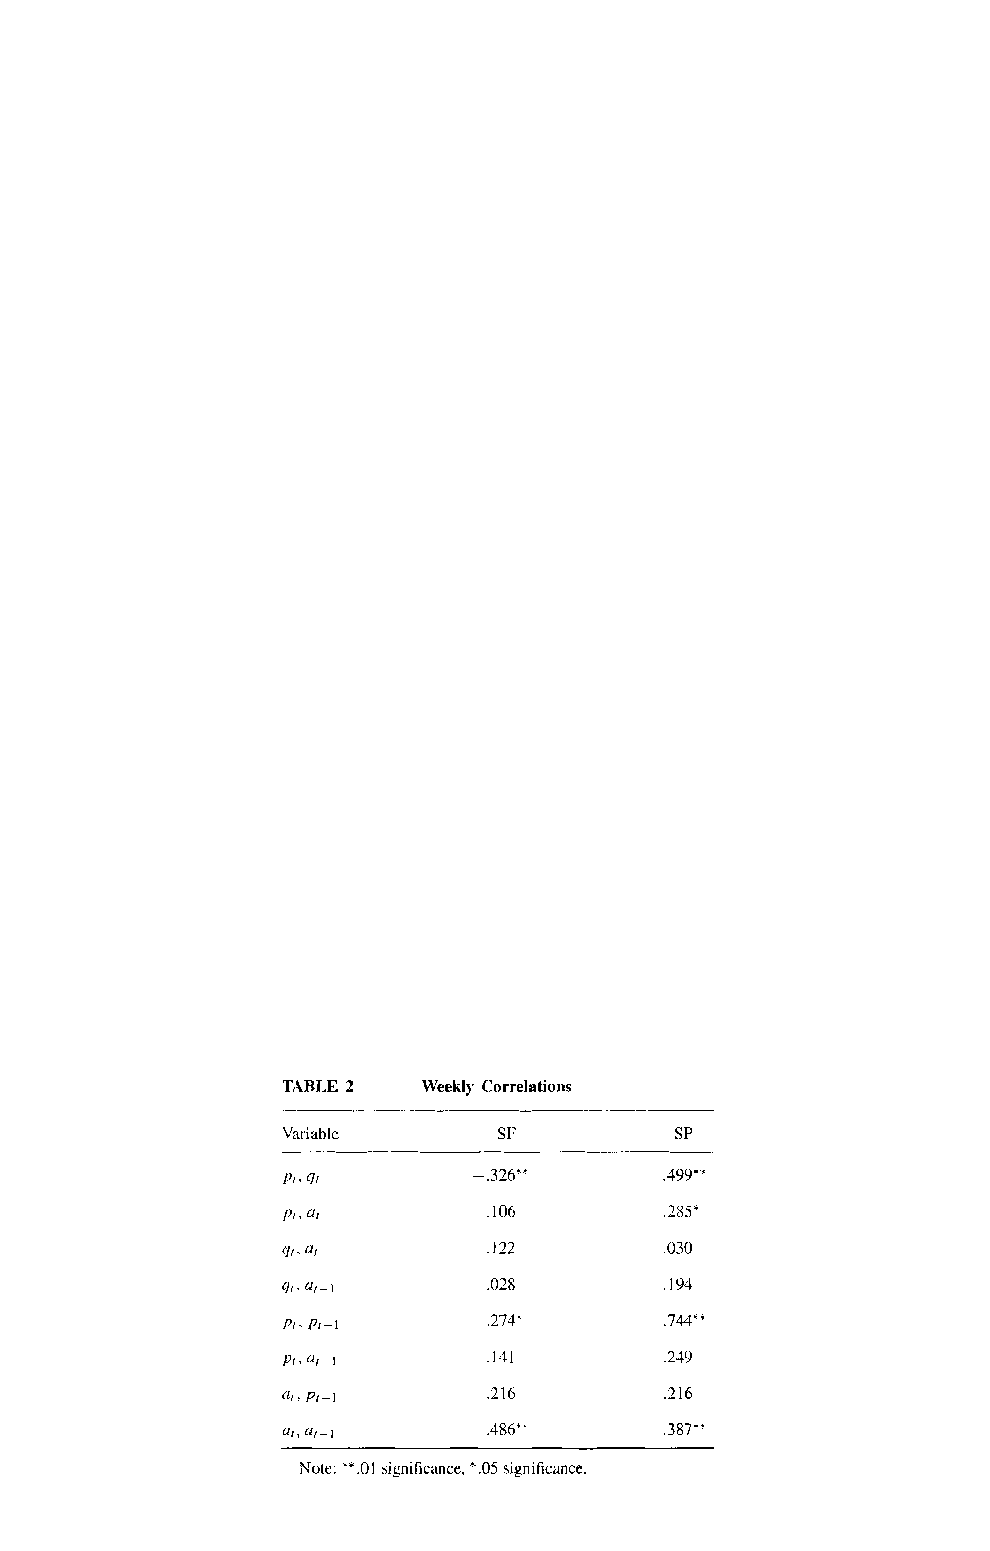
\includegraphics[width=9.5cm]{resources/acker2.pdf}
\label{default}
\end{center}
\end{figure}
\end{frame}

\begin{frame}{Table 3: Descriptive Results}
\begin{figure}[htbp]
\begin{center}
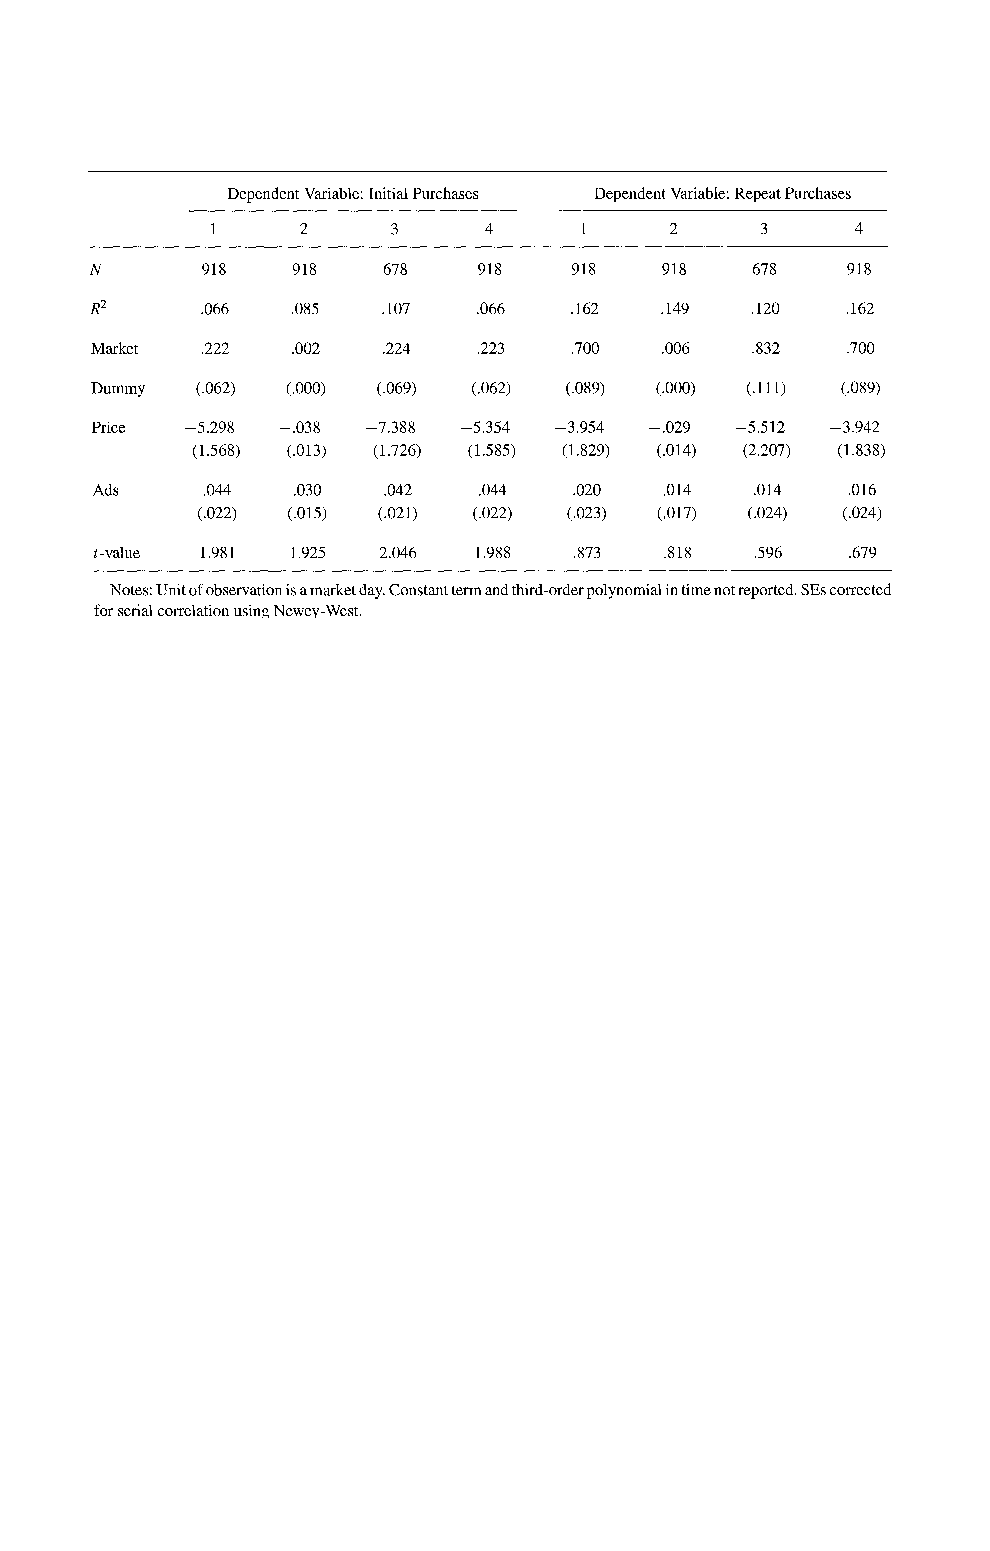
\includegraphics[width=9.5cm]{resources/acker3.pdf}
\label{default}
\end{center}
\end{figure}
\end{frame}



\begin{frame}{Model}
Reduced form for discrete choice that consumer $i$ purchases Yoplait 150 on trip $t$
\begin{eqnarray*}
c_{it} = \begin{cases}
       1 & \mbox{ IFF } \alpha_i + X_{it} \beta_1 - \gamma p_{it} + \epsilon_{1it} > Z_{it} \beta_2 + \epsilon_{2it}\\
       0 & \mbox{ o.w. } 
        \end{cases}
\end{eqnarray*}
\begin{itemize}
\item First term may \alert{proxy} for static utility or choice specific value function of YP150 purchase
\item Second term represents utility of outside option
\item $\alpha_i$ is a random effect (persistent heterogeneity) for YP150.
\item $X_{it}$ contains \alert{advertising}, household and consumer characteristics, and functions of previous purchases of YP150, coupon, time trend.
\item $Z_{it}$ contains an index of other competitors' prices
\end{itemize}
\end{frame}

\begin{frame}{Likelihood}
\begin{eqnarray*}
L_i(\theta) &=& Pr[c_{i1},\ldots,c_{iT_i} | W_i^t, Z_i^t, p_i^t; \theta] \\
&=& \int Pr[c_{i1},\ldots,c_{iT_i} | W_i^t, Z_i^t, p_i^t; a_i;  \theta] f(d \alpha_i | \theta)\\
&=& \int \prod_{t=1}^{T_i} Pr[c_{it}|  X_{it}(c_{i}^{t-1}), Z_{it}, p_{it}; a_i;  \theta] f(d \alpha_i | \theta)
\end{eqnarray*}
\begin{itemize}
\item $c_{i}^{t-1}$ is your entire purchase history
\item $W_{i}^t$ is the subset of explanatory variables $X_{it}$ that are completely exogenous
\item Choice probabilities determined by $\epsilon$ IID logit.
\end{itemize}
\end{frame}

\begin{frame}{Table 4: Parameter Estimates}
\begin{figure}[htbp]
\begin{center}
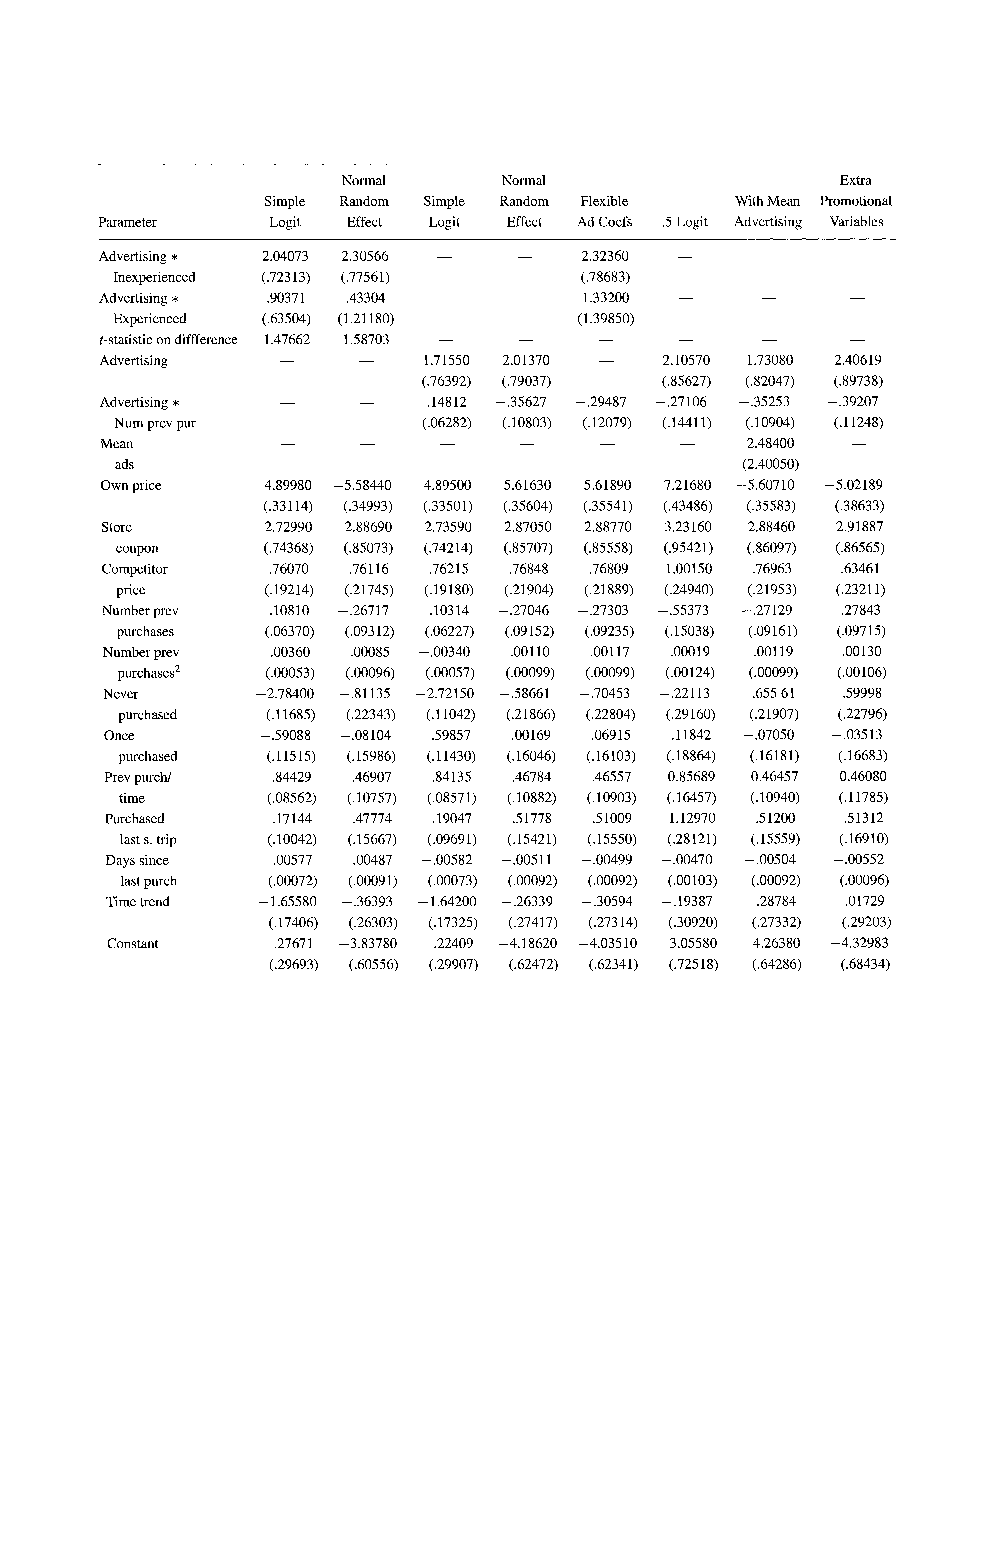
\includegraphics[width=8.5cm]{resources/acker4.pdf}
\label{default}
\end{center}
\end{figure}
\end{frame}

\begin{frame}{Discussion}
\begin{itemize}
\item Adv*Exp \alert{insignificant} image and prestige
\item Adv*Inexp - Adv*Exp: \alert{significant} informative
\item 30-sec commercial each week is like 10 cent price decrease
\item Adv*NPurch: decreasing returns to advertising
\end{itemize}
\end{frame}

\section*{Erdem and Keane}

\begin{frame}{Erdem Keane}
\begin{itemize}
\item Many markets are characterized by lots of new brands, price changes, and brand repositioning (especially CPG).
\item Nevo (2001) has hundreds of cereal brands enter and exit, similar in laundry detergent
\item Consumers may spend time experimenting with different brands to learn about them.
\item After learning takes place there may be state dependence until new brands are introduced or price cuts.
\end{itemize}
\end{frame} 

\begin{frame}{Guardini Little (Pre-Dynamics)}
\begin{eqnarray*}
E[U_{ij} | I_i(t) ] = a_j -w_P P_j + w_E \sum_{s=0}^t D_{1ijs}  + w_{Ad} \sum_{s=t_0}^t D_{2ijs}
\end{eqnarray*}
\begin{itemize}
\item $a_j$ mean brand taste for $j$
\item $D_{1ijt}$: dummy of whether consumer purchases brand $j$ or not
\item $D_{2ijt}$: dummy of whether consumers receives an advertising signal of brand $j$ or not
\item $w$ are utility weights (Lancaster 1966)
\end{itemize}
\end{frame} 


\begin{frame}{Erdem Keane: Decision-making Under Uncertainty}
\begin{itemize}
\item Consumer $i$ chooses among $J$ products in $T$ periods of time.
\item $d_{ij}(t)=1$ if consumer chooses $j$ (0 o.w.)
\item Includes an \textit{other brand} option
\item $E[U_{ij}(t) | I_i(t)]$ is current period expected utility conditional on information set $I_i(t)$.
\end{itemize}
Consumers maximize a discounted stream of expected utilities producing the Bellman:
\begin{eqnarray*}
V_{ij}(I_i(t),t) &=& E[U_{ij}(t) | I_i(t)] + \beta E[V(I(t+1),t+1) | I(t)] \\
V_i(I(t),t) &=& \max_j V_j(I_j(t),t)
\end{eqnarray*}
\end{frame}


\begin{frame}{Attribute Uncertainty}
\begin{itemize}
\item $A_{ijt} = A_j + \xi_{ijt} $ with i.i.d. mean zero shock $\xi_{ijt}$
\item Consumers don't immediately learn about attribute levels, instead:
\item $A_{E_{ijt}} = A_{ijt} + \eta_{ijt}$ with mean zero i.i.d disturbance $\eta_{ijt}$.
\item $A_{E_{ijt}} = A_{j} + \delta_{ijt}$ where $\delta_{ijt} = \xi_{ijt} + \eta_{ijt}$.
\item Empirically can't differentiate between private value $\xi_{ijt}$ and experience shock $\eta_{ijt}$.
\end{itemize}
\end{frame}

\begin{frame}{Consumer Expected Utility}
Additive Compensatory Multiattribute utility model. (Fishbein 1967) (Lancaster 1966)
\begin{eqnarray*}
U_{ijt} &=& -w_p P_{ijt} + w_A A_{E_{ijt}} - w_A r A_{E_{ijt}}^2 + e_{ijt}\\
E[U_{ijt} | I_i(t)] &=& -w_j P_{ijt} + w_A E[A_{E_{ijt}} | I(t)] - w_A r E [A_{E_{ijt}} | I_i(t)]^2\\
&&-w_A r E[A_{E_{ijt}} - E[A_{E_{ijt}}^2 | I_i(t)]]^2 + e_{ijt}
\end{eqnarray*}
Where $r$ is your risk parameter:  $r > 0$ risk averse
\begin{eqnarray*}
EU_{i0t}  &=& \Phi_{O} + \Phi_{Ot} + \epsilon_{i0t}\\
EU_{iNPt}  &=& \Phi_{NP} + \Phi_{NPt} + \epsilon_{iNPt}
\end{eqnarray*}
For outside good or other good.
\end{frame}

\begin{frame}{Bayesian Learning}
With no experience initial variability $\delta_{ijt}$, and advertising signal $S_{ijt}$
\begin{eqnarray*}
\delta_{ijt} \sim N(0,\sigma_{\delta}^2),  \quad& A_j \sim N(A,\sigma_A^2(0))\\
S_{ijt} = A_j + \zeta_{ijt}, \quad &\zeta_{ijt} \sim N(0,\sigma_{\zeta}^2)
\end{eqnarray*}
Consumers update:
\begin{eqnarray*}
E[A_{E_{ij,t+1}} | I_i(t)] &=&  E[A_{E_{ijt}} | I_i(t-1)] \\
 &-& D_{1ijt} \beta_{1ij}(t) [A_{E_{ijt}} - E[A_{E_{ijt}} | I_i(t-1)] ] \\
 &+&D_{2ijt} \beta_{2ij}(t) [S_{E_{ijt}} - E[S_{E_{ijt}} | I_i(t-1)] ] \\
\end{eqnarray*}
\end{frame}

\begin{frame}{Bayesian Learning}
\begin{itemize}
\item $D_{1ijt}$: dummy of whether consumer purchases brand $j$ or not
\item $D_{2ijt}$: dummy of whether consumers receives an advertising signal of brand $j$ or not
\item Kalman Filter Update
\begin{eqnarray*}
\beta_{1ijt} = \frac{ \sigma_{vij}^2(t)} { \sigma_{vij}^2(t) + \sigma_{\delta}^2}, &\quad& 
\beta_{2ijt} = \frac{ \sigma_{vij}^2(t)} { \sigma_{vij}^2(t) + \sigma_{\zeta}^2}\\
v_{ij} &=& E[A_{ij} | I_{ij}(t)] - A_j
\end{eqnarray*} 
\item And
\begin{eqnarray*}
A_{j} &=& E[A_j | I_{ij}(t)] + v_{ij}(t)\\
A_{E_{ijt}} &=& A_j + \delta_{ijt} , \quad S_{ijt} = A_j + \zeta_{ijt}
\end{eqnarray*} 
\end{itemize}
\end{frame}

\begin{frame}{Bayesian Learning}
\begin{eqnarray*}
v_{ijt}(t) &=& v_{ij}(t-1) + D_{1ijt} \beta_{1ij}(t)[-v_{ij}(t-1) + \delta_{ijt}]  \\
&+& D_{2ijt} \beta_{2ij}(t)[-v_{ij}(t-1) + \zeta_{jt}]\\
\sigma_{vij}^2(t) &=& \frac{1}{\frac{1}{\sigma_v^2(0)} + \frac{\sum_{s=0}^t D_{1ijs}}{\sigma_{\delta}^2} + \frac{\sum_{s=0}^t D_{2ijs}}{\sigma_{\zeta}^2}}
\end{eqnarray*}
And expected utilities:
\begin{eqnarray*}
E[U_{ij} | I_i(t)] &=& w_A A_j - w_A r A_j^2 -w_A r \sigma_{\delta}^2 -w_P P_{ij} \\
&-& -w_A r \sigma_{vij}^2(t) - w_A r v_{ij}(t)^2  - w_A v_{ij}(t) - 2w_A r A_j v_{ij} (t) \\ &+& e_{ijt}\\
E[V_{ij} | I_i(t)] &=& E[U_{ij} | I_i(t)] + \beta E[V_{ij} | I_i(t+1) | d_{ijt} =1, I_i(t)]
\end{eqnarray*}
\end{frame}


\begin{frame}{Choice Probabilities}
For the Static and Dynamic case:
\begin{eqnarray*}
P^s_i(I(t),t) = \int \frac{\exp [E [U_{ij} | I_i(t)] ] } {\sum_k \exp [E [U_{ik} | I_i(t)] ] } f(v) dv\\
P^d_i(I(t),t) = \int \frac{\exp [E [V_{ij} | I_i(t)] ] } {\sum_k \exp [E [V_{ik} | I_i(t)] ] } f(v) dv
\end{eqnarray*}
\begin{itemize}
\item Static model allows choices to depend on 
\alert{current knowledge of attribute}
\item Static model does not incorporate \alert{value of learning for future consumption}
\item Logit choice probabilities but with time varying random coefficients
\item Everything about learning in is in the distribution of $v$
\end{itemize}
\end{frame}


\begin{frame}{Data}
\begin{itemize}
\item Laundry detergent scanner data from 1986-1988.
\item 3000 HH's w/ 20 purchases (7 liquid)
\item Lots of advertising
\item Only liquids (80\% of market)
\item Many new brands
\item  TVs measures ad exposure
\begin{itemize}
\item Percentage of weeks household saw brand $j$'s ad.
\item Saw at least one ad during that week
\end{itemize}
\end{itemize}
\end{frame}


\begin{frame}{Table 2: Static Model No Learning} 
\begin{figure}[htbp]
\begin{center}
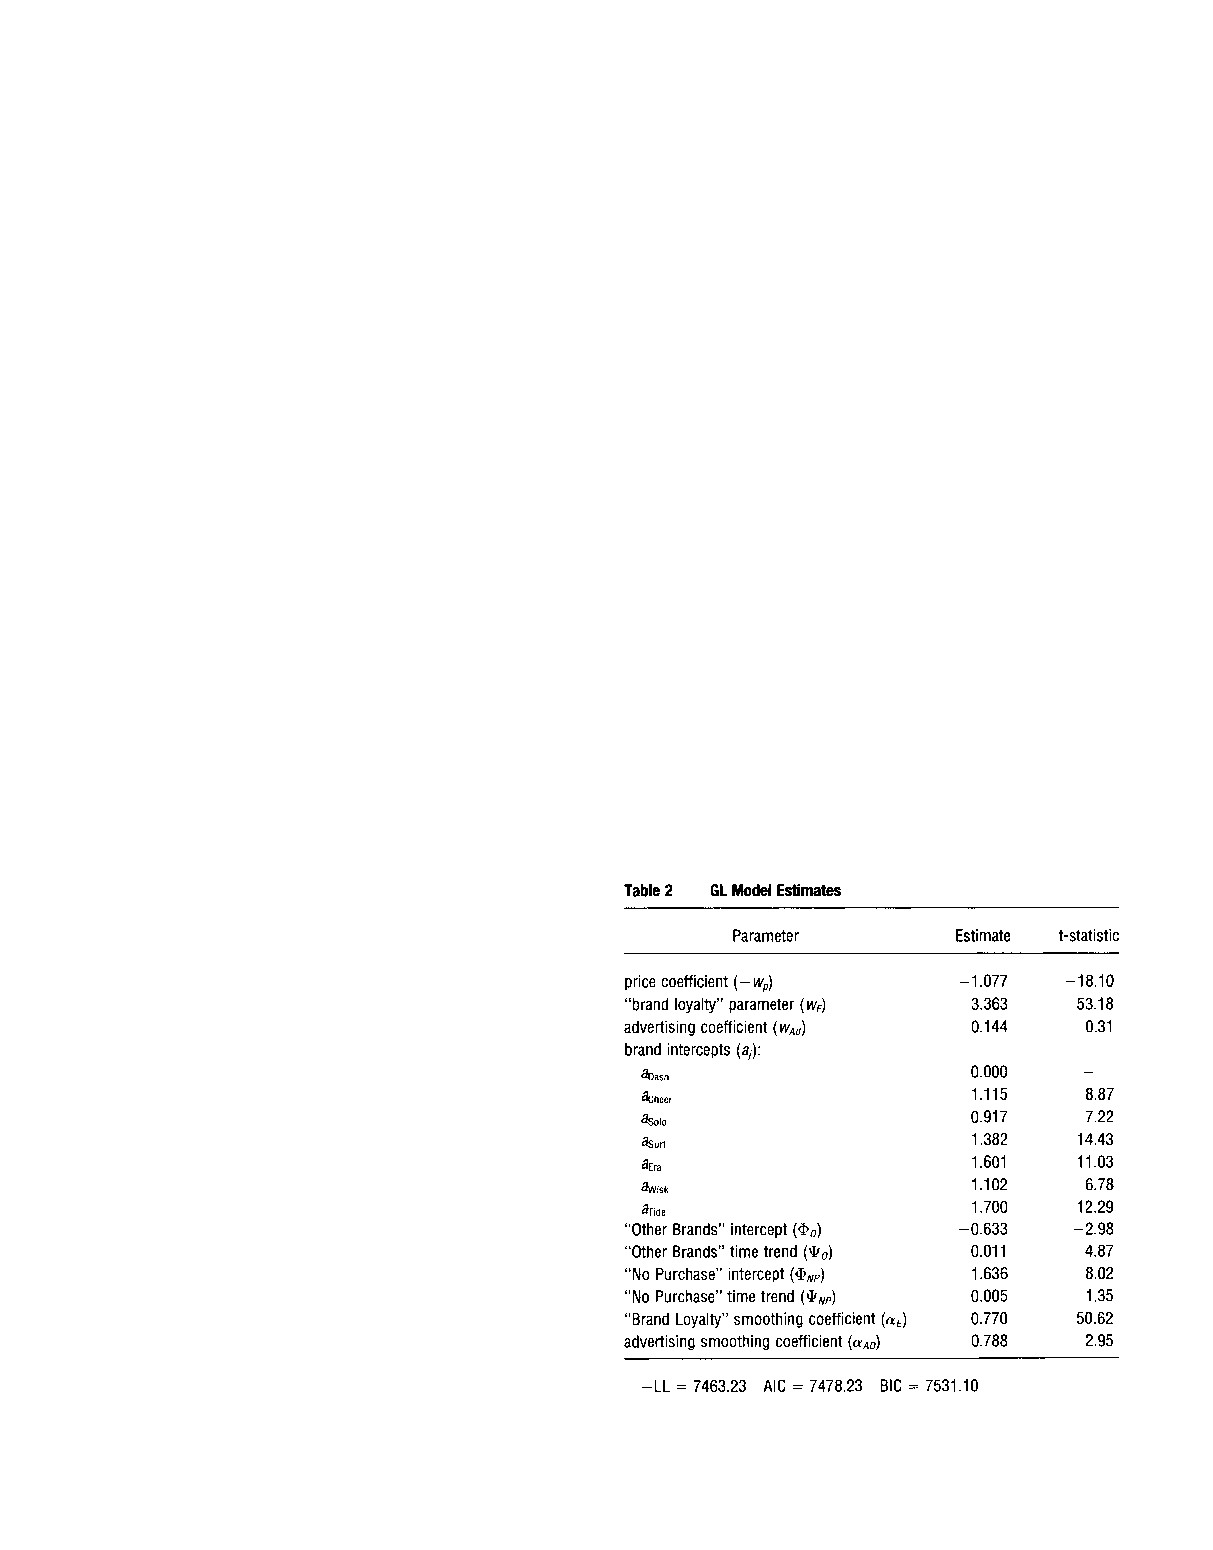
\includegraphics{resources/ek1.pdf}
\label{default}
\end{center}
\end{figure}
\end{frame}

\begin{frame}{Table 3: Dynamic Model}
\begin{figure}[htbp]
\begin{center}
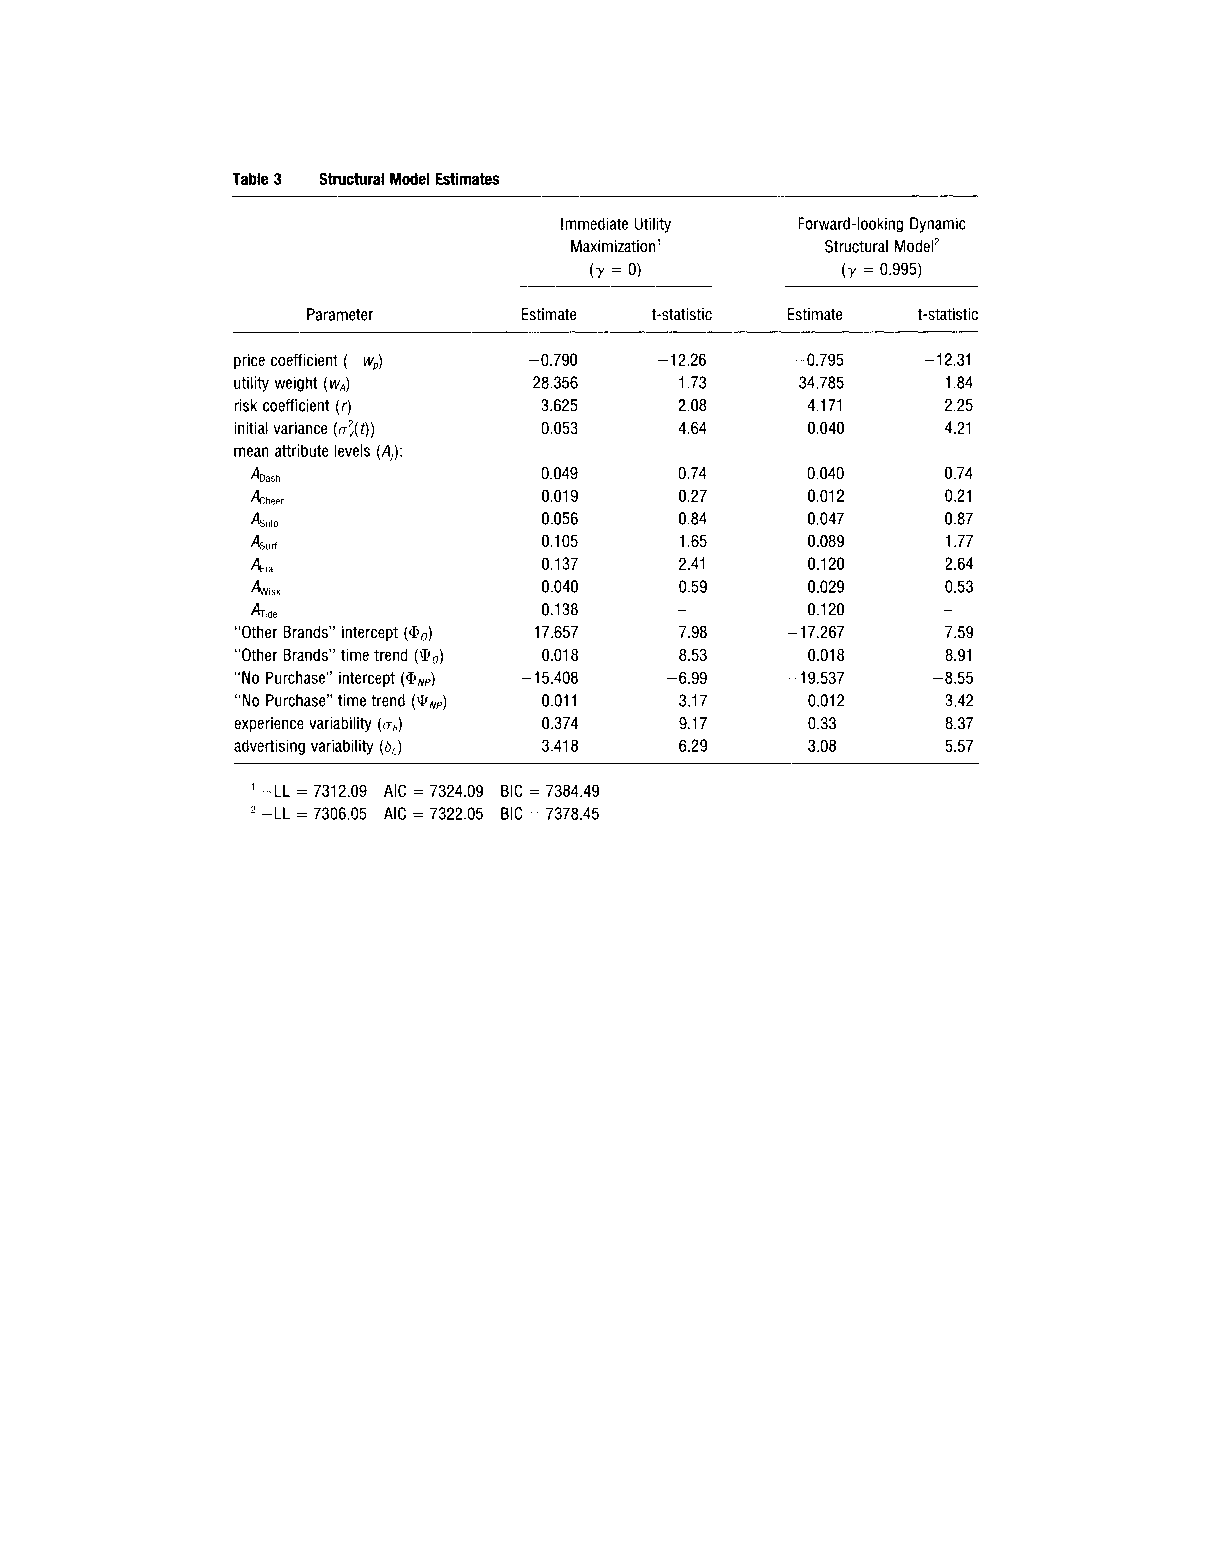
\includegraphics[width=4in]{resources/ek2.pdf}
\label{default}
\end{center}
\end{figure}
\end{frame}

\begin{frame}{Results}
\begin{itemize}
\item Static model has no effect of advertising (!)
\item Consumers are risk averse
\item Price coefficient negative and significant
\item Utility weight is huge (latent attribute -- cleaning power?)
\item Attribute levels are not significant (maybe differences are?)
\item Advertising more variable than experience
\item relatively small initial variance
\item Dynamic model shows \alert{more willingness to try new brands}
\end{itemize}
\end{frame}

\section*{Crawford and Shum}

\begin{frame}{Uncertainty and Learning in Pharmaceutical Demand}
Crawford and Shum (2005)
\begin{itemize}
\item  Italian anti-ulcer data: 34,972 patients (and a total of 98,634 prescription episodes)
\item Patients receive, on average, $2.8$ prescriptions for $1.2$ drugs over a period of just under 6 months.
\item Break up data into \textit{spells} or a sequence of one or more prescriptions of a single drug.
\begin{itemize}
\item A patient has 1.2 spells on average
\item An average spell is around 2.37 prescriptions
\end{itemize}
\item Probability of switching drugs is not constant over time
\begin{enumerate}
\item Early Switching: \alert{Experimentation} - about 10\% after first prescription
\item Late Switching: \alert{Learning} rise in switching at the end, especially for long-treatment length patients
\end{enumerate}
\end{itemize}
\end{frame}


\begin{frame}{Uncertainty and Learning in Pharmaceutical Demand}
\begin{figure}[htbp]
\begin{center}
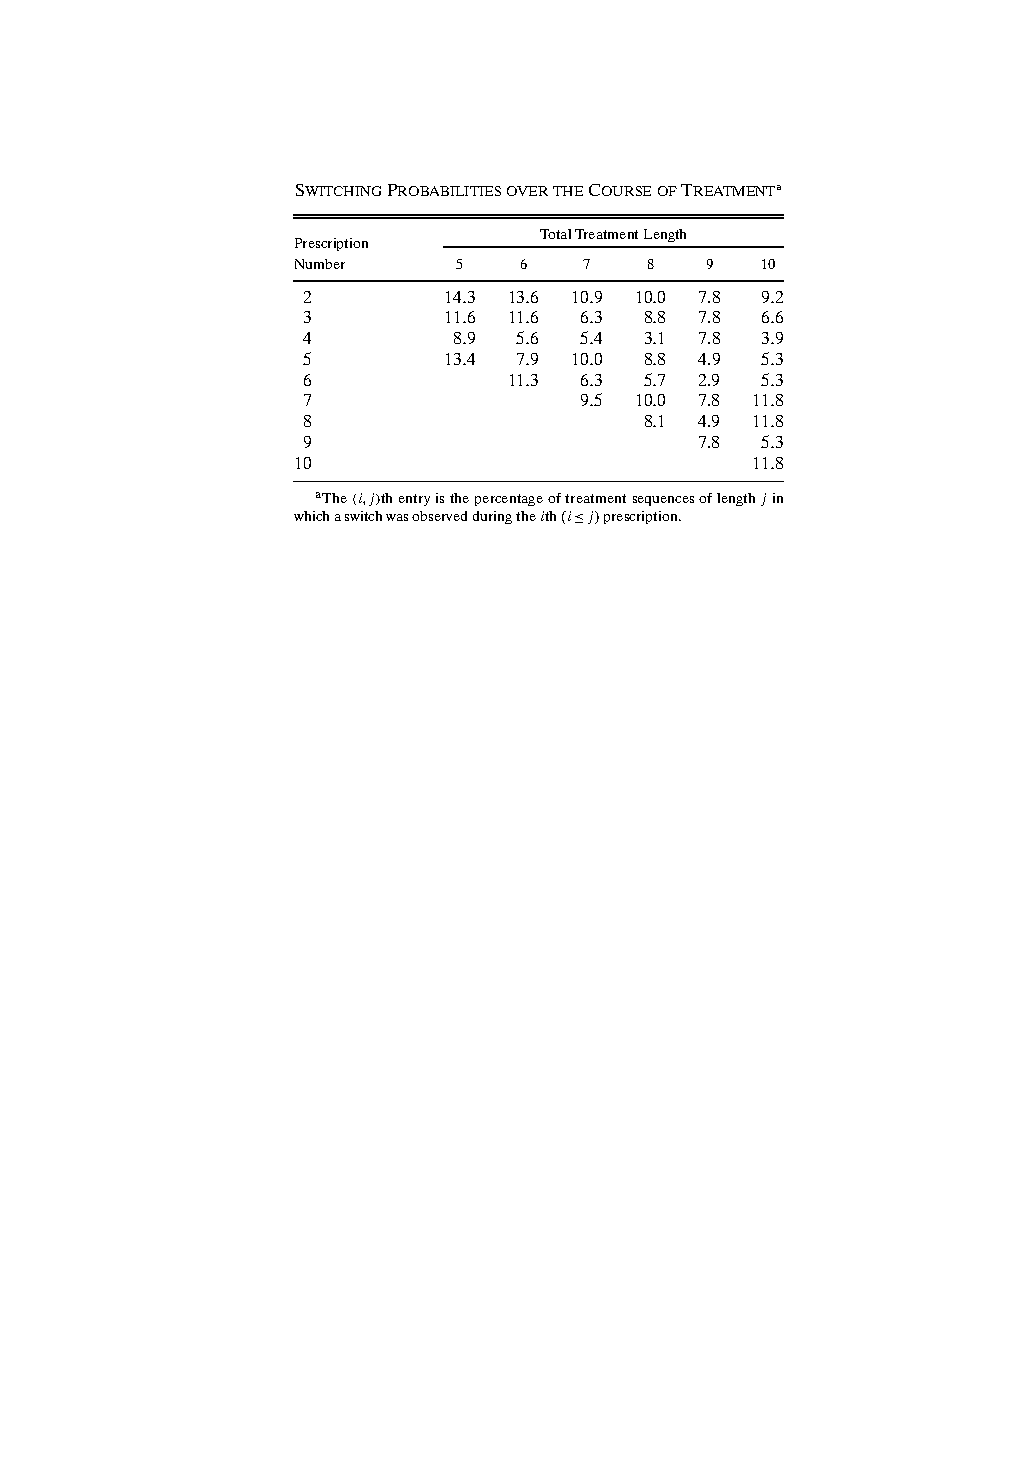
\includegraphics{resources/crawfordshum1.pdf}
\label{default}
\end{center}
\end{figure}
\end{frame}

\begin{frame}{Model Setup}
\begin{itemize}
\item Patients, $j$. Drugs, $n=5$, types $k=4$ (known to doctor-patient but not econometrician).
\item Treatment is characterized by two match values $(\mu_{jn},\nu_{jn})$ and two corresponding signals $(x_{jnt},y_{jnt})$ that correspond to the side-effects or curative probabilities respectively.
\item Patient's utility $u(\cdot)$ depends on side effects $x_{int}$
\item Cure probability $w(\cdot)$ depends on $y_{jnt}$
\item Don't know your match value  $(\mu_{jn},\nu_{jn})$  only the signal $(x_{jnt},y_{jnt})$, or treatment length $\tau = 1,\ldots,T$
\end{itemize}
\end{frame}


\begin{frame}{Model Setup}
\begin{itemize}
\item Consumers have both signals $(x,y)$ and priors $(\mu,\nu)$ about side effects and cure probability
\begin{eqnarray*}
\left( \begin{smallmatrix} x_{jnt} \\ y_{jnt} \end{smallmatrix} \right)
&\sim& N \left( \begin{smallmatrix} \mu_{jn} \\ \nu_{jnt} \end{smallmatrix}, \begin{smallmatrix} \sigma^2_{jn} \\ \tau_{jnt}^2 \end{smallmatrix} \right) \\
\left( \begin{smallmatrix} \mu_{jn} \\ \nu_{jn} \end{smallmatrix} \right)
&\sim& N \left( \begin{smallmatrix} \overline{\mu}_{nk} \\ \overline{\nu}_{nk} \end{smallmatrix}, \begin{smallmatrix} \overline{\sigma}^2_{n} \\ \overline{\tau}_{n}^2 \end{smallmatrix} \right)
\end{eqnarray*}
\item Where $k=1,\ldots,4$ indexes the \alert{type specific priors}. 
\end{itemize}
\end{frame}

\begin{frame}{Model Setup}
\begin{itemize}
\item Doctors (without incentive problems) solve:
\begin{eqnarray*}
\max_{D=\{(d_{jnt})_{n=1}^N \}_{t=1}^{\infty}} E_D \sum_{t=1}^{\infty} \beta^t d_{jnt} u_{jnt}(1 - w_{j,t-1})
\end{eqnarray*}
\item Patients have CARA utility
\begin{eqnarray*}
u(x_{jnt},p_n,\epsilon_{jnt}) &=& -\exp(r *x_{jnt}) - \alpha p_n + \epsilon_{jnt}
\end{eqnarray*}
\item Derive the expected utility as:
\end{itemize}
\vspace{-0.5cm}
\begin{eqnarray*}
\tilde{EU}(\mu_{jn}(t),\nu_{jn}(t), p_n,\epsilon_{jnt}) &=& -\exp(r *\mu_{jn}(t) + \frac{1}{2} r^2(\sigma) (\sigma^2_n + V_{jn}(t))) \\
&& - \alpha p_n + \epsilon_{jnt}\\
&=& EU(\mu_{jn}(t),V_{jn}(t),p_n) + \epsilon_{jnt}
\end{eqnarray*}
\end{frame}

\begin{frame}{State Space}
\begin{itemize}
\item State Variables $S_t$:
\begin{itemize}
\item $(\mu_{jnt},\nu_{jnt}), I_{jnt}$ for $n=1,\ldots,5$ drugs.
\item $h_{j,t-1}$ (cure probability)
\item $\epsilon_{jnt}$
\end{itemize}
\item Recovery probability follows a Markov Process:
\begin{eqnarray*}
h_{jt}(h_{j,t-1},y_{jnt}) = \frac{ \left(\frac{h_{j,t-1}}{1-h_{j,t-1}} \right) + d_{jnt} y_{jnt}}  {1+ \left(\frac{h_{j,t-1}}{1-h_{j,t-1}} \right) + d_{jnt} y_{jnt}}  
\end{eqnarray*}
\item Beliefs follow Bayesian updating depending on $I_{jnt}$ the number of times patient $j$ takes drug $n$ at time $t$.
\end{itemize}
\end{frame}

\begin{frame}{Dynamic Decision Problem (DDP)}
Doctors face choice specific value function (infinite horizon, recovery state absorbing):
\begin{eqnarray*}
W(S_t) &=& \max_n [\exp(-r\mu_{jnt} + 0.5r^2(\sigma_n^2 + V_{jnt})) - \alpha p_n + \epsilon_{jnt}\\
&&+ \beta E[(1-h_{jt}(h_{j,t-1},y_{jnt}) E[W(S_{t+1}) | x_{jnt},y_{jnt},d_n=1] | S_t]\\
&=& \log [ \sum_n \exp[ \tilde{EU}(s) + \beta E[(1-h(s'))W(s') | d_n=1] | S_t] \\
&=& \max_n \{W_n(S_t)\}
\end{eqnarray*}
\end{frame}

\begin{frame}{Value Function}
\begin{eqnarray*}
W(S_t) &=& \max_n [\exp(-r\mu_{jnt} + 0.5r^2(\sigma_n^2 + V_{jnt})) - \alpha p_n + \epsilon_{jnt}\\
&&+ \beta E[(1-h_{jt}(h_{j,t-1},y_{jnt}) E[W(S_{t+1}) | x_{jnt},y_{jnt},d_n=1] | S_t]\\
&=& \log [ \sum_n \exp[ \tilde{EU}(s) + \beta E[(1-h(s'))W(s') | d_n=1] | S_t] \\
&=& \max_n \{W_n(S_t)\}
\end{eqnarray*}
\end{frame}

\begin{frame}{VFI + Simulate + Interpolate: (Keane Wolpin 1994): }
\begin{enumerate}
\item Define discrete grid $S^* \in S$
\item For each state $s \in S^*$ make an initial guess at the value function $W^0(s)$.
\item Run regression $W^0(s) = G(s)'\theta^0 + \varepsilon$
\item Draw the $M$ random signals $\{x_{jn}^m, y_{jn}^m\}$
\item Compute the expected value of choosing drug $n$ for each $s \in S^*S$, where $s^m$ is state corresponding to random draw $m$ and drug $n$ being chosen.
\begin{eqnarray*}
E[W(s | d_n =1,s)] = \frac{1}{M} \sum_m (1-h(s^m)) W^0(s^m)
\end{eqnarray*}
\item Update the value function for each $s \in S^{*}$
\item Iterate until convergence
\end{enumerate}
\end{frame}

\begin{frame}{Likelihood}
For $I_=0$ and $I_j=1$ censored and uncensored observations for patient $j$.
\begin{eqnarray*}
&&\sum_{k=1}^K p_k E_{\overline{x}_{jn T_{j}},k | h_{0,j,k}} \left[ \prod_{t=1}^{T_j-1} \left((1-h_{jt,k}) \prod_n \lambda_{jnt,k}^{d_{jnt}} \right) \right] \cdot h_{jT_j,k} \prod_n  \lambda_{jnt,k}^{d_{jnt}}\\
&&\sum_{k=1}^K p_k E_{\overline{x}_{jn T_{j}},k | h_{0,j,k}} \left[ \prod_{t=1}^{T_j-1} \left((1-h_{jt,k}) \prod_n \lambda_{jnt,k}^{d_{jnt}} \right) \right] \cdot \prod_n  \lambda_{jnt,k}^{d_{jnt}}\\
\end{eqnarray*}
($\lambda$ is logit choice probability)\\
We need to calculate expectations of joint distribution of $(\overline{x},h)$ by drawing $S=30$ sequences  per patient.
\end{frame}

%--------------------------------------------------------------------------------

\begin{frame}
\frametitle{Identification}

\begin{itemize}
\item Key restrictions

\begin{itemize}
\item drug's symptomatic effects only impact a patient's utility

\item curative effects only influence the recovery probabilities
\end{itemize}

\item For $(\underline{\mu }_{j},\underline{\sigma }_{j}^{2},\sigma _{j},r)$

\begin{itemize}
\item enter per period utility expression

\item $\underline{\mu }_{j}$ comes from initial prescription shares across
patients

\item Difference in drug choice probabilities early vs. late in sequence
help identify $\underline{\sigma }_{j}^{2}$

\item $r$ vs. $\sigma _{j}$

\begin{itemize}
\item persistence in drug choices gives r

\item extent to which rate of switching varies with $l_{ij}^{t}$ identifies $%
\sigma _{j}$
\end{itemize}
\end{itemize}
\end{itemize}
\end{frame}

%--------------------------------------------------------------------------------

%--------------------------------------------------------------------------------

\begin{frame}
\frametitle{Identification}

\begin{itemize}
\item For $(\underline{\nu }_{j},\underline{\tau }_{j}^{2},\tau _{j},h_{0i})$

\begin{itemize}
\item enters dynamic choice problem through expected recovery probability

\item $h_{0i}$ identified separately because it only enters healing
probability; other 3 enter posterior mean and variance for curative match
value
\end{itemize}

\item Can identify $\underline{\mu }_{j}$ separately from price coefficient, 
$\alpha $, because of functional form assumption; $\underline{\mu }_{j}$
enters per period utility nonlinearly and $\alpha $ enters linearly.
\end{itemize}
\end{frame}


\begin{frame}{Dynamic Model Parameters: Sick vs. Not so Sick}
\begin{figure}[htbp]
\begin{center}
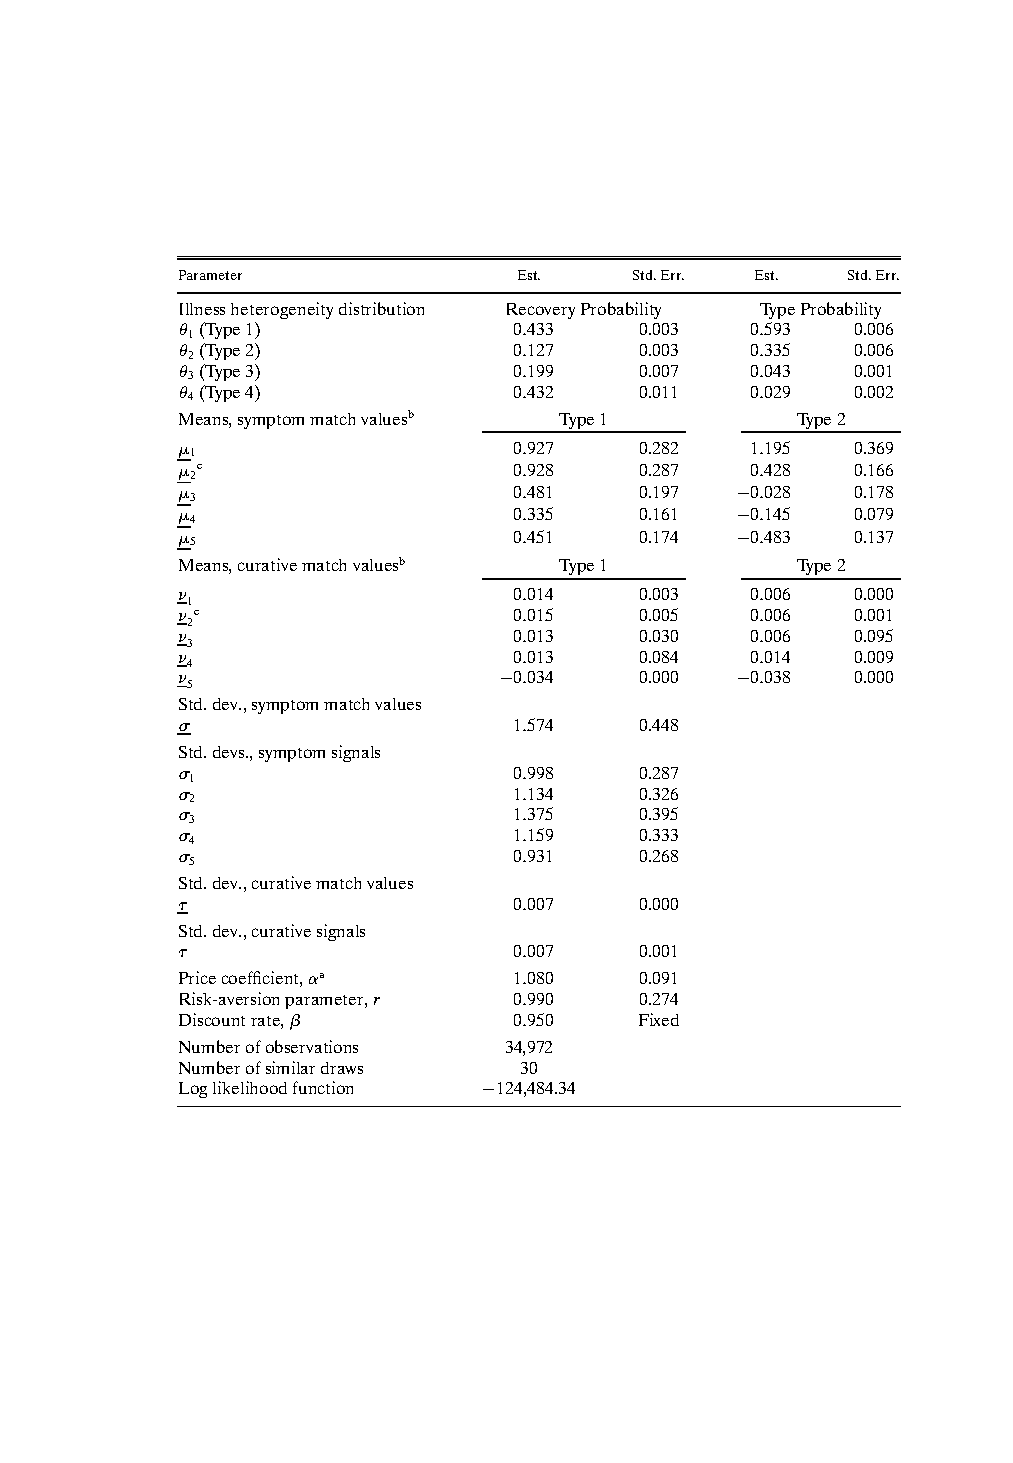
\includegraphics[width=7cm]{resources/crawfordshumparam.pdf}
\label{default}
\end{center}
\end{figure}
\end{frame}

\begin{frame}{Dynamic Model Parameters: Omeprazole (All types)}
\begin{figure}[htbp]
\begin{center}
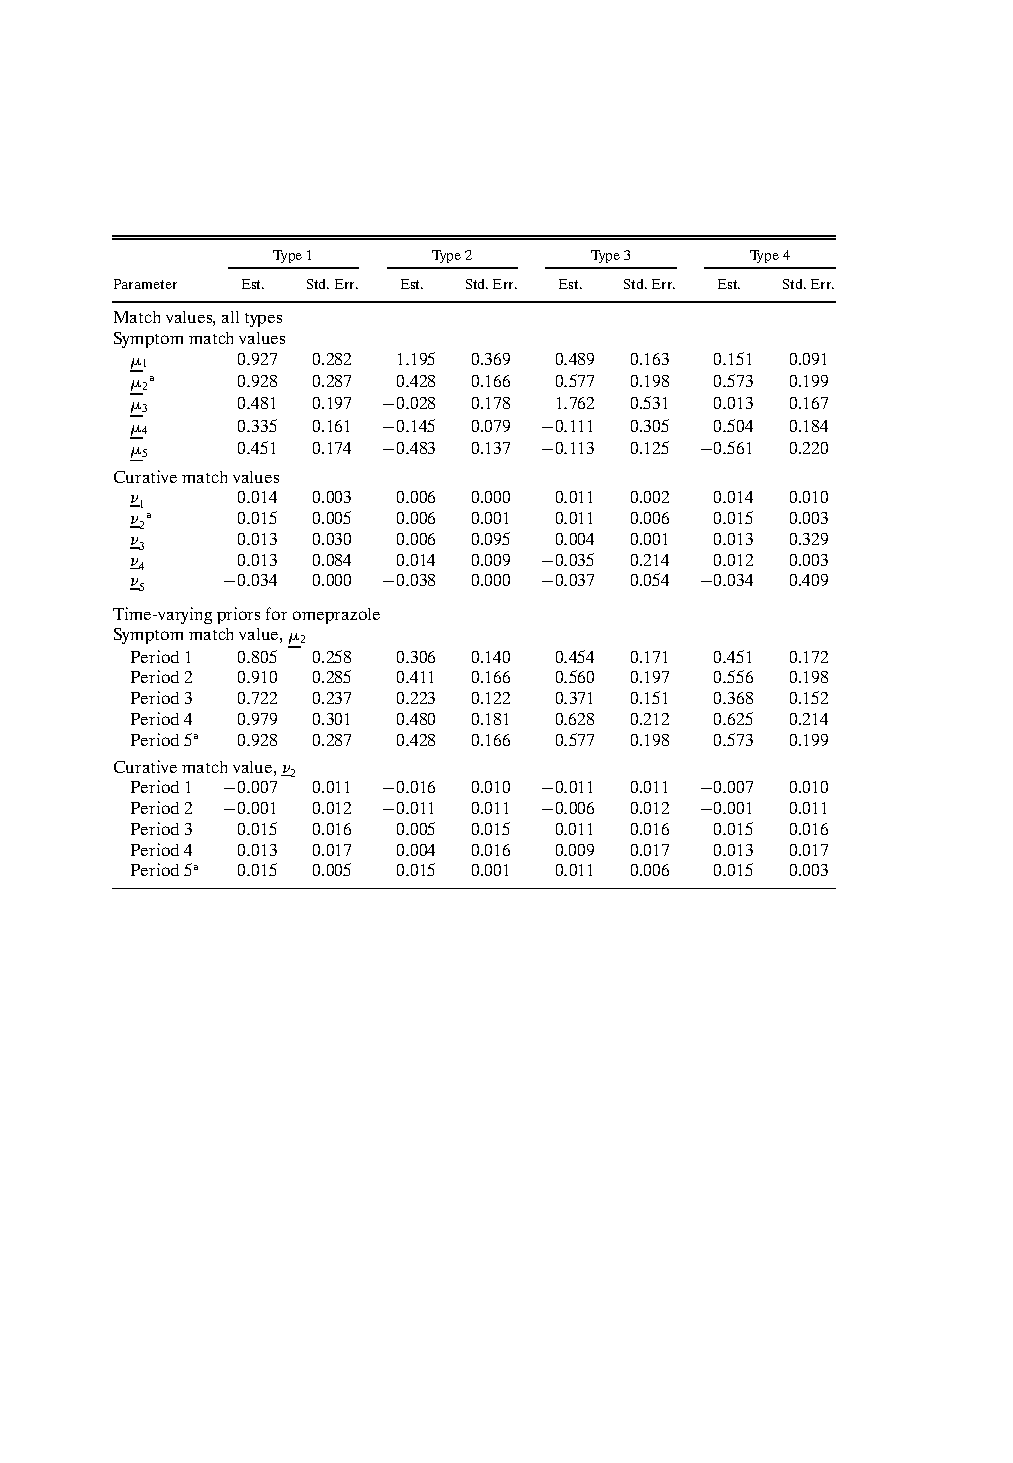
\includegraphics[width=7cm]{resources/crawfordshumparam2.pdf}
\label{default}
\end{center}
\end{figure}
\end{frame}

\begin{frame}{Results}
\begin{itemize}
\item Coefficient of risk aversion is high (switching costs?)
\item Learning happens very fast (variance falls from 2.48 to 0.7 after only \alert{one prescription}).
\item Learning slows after first prescription
\item Counterfactual (Complete Information): You know your match values which you draw from the same distribution but your perceived variance $V_{jn}^t = R_{jn}^=0$.
\begin{itemize}
\item Leads to more drugs $1.9$ instead of $1.4$.
\item Substitution away from market leader (no reason to stay with first drug). Lower HHI
\item Welfare up 9\%. Treatment up 80\%, cost up 60\%.
\end{itemize}
\item Counterfactual (Ban Experimenting): You are stuck with your first drug forever.
\begin{itemize}
\item Utility down 6\% but treatment length and costs about the same.
\item Wasn't much experimentation to begin with
\end{itemize}
\item Counterfactual (No Diagnostic Matching): Doctors can't learn types.
\begin{itemize}
\item Utility down 11\% and costs and length up 30-40\%.
\end{itemize}
\end{itemize}
\end{frame}





%--------------------------------------------------------------------------------

%--------------------------------------------------------------------------------

\begin{frame}
\frametitle{Results}

\begin{itemize}
\item Counterfactual 1: patients have complete info about match values (set
perceived variances, $(V_{ij}^{t},R_{ij}^{t})\,=0$)

\begin{itemize}
\item discounted expected utility increases (though by small amount)

\item average number of drugs used increases
\end{itemize}

\item Counterfactual 2: constrain patients to take the first drug they're
prescribed

\begin{itemize}
\item shuts down learning after 1st prescription

\item does not change simulated treatment lengths

\item lowers avg utility 6\%
\end{itemize}

\item Counterfactual 3: no diagnostic matching to patient "type"

\begin{itemize}
\item expected utility decreases 11\%, costs 40\% higher than baseline

\item diagnostic matching at least as important as idiosyncratic learning
\end{itemize}
\end{itemize}
\end{frame}

%--------------------------------------------------------------------------------

%--------------------------------------------------------------------------------


\section{Dickstein: Efficient Provision of Experience Goods: Evidence from
Antidepressant Choice}


%--------------------------------------------------------------------------------

\section{Goals and RQ}

%--------------------------------------------------------------------------------

\begin{frame}
\frametitle{Goals of Paper}

\begin{itemize}
\item Theory Testing

\item Measurement

\item Methodology
\end{itemize}
\end{frame}

%--------------------------------------------------------------------------------

\begin{frame}
\frametitle{Goals of the Paper}

\begin{itemize}
\item Theory Testing

\begin{itemize}
\item Do the pricing schemes of Shapiro (1983), Bergemann and Valimaki
(2006) appear in markets in which consumer perceptions change with
experience?

\item Can adherence information in observational data provide a measure of
treatment effectiveness?
\end{itemize}

\item Measurement

\begin{itemize}
\item Identify the elasticity of patients/physicians with respect drug
copayments and wholesale prices

\item Measure the dynamic response of patients and physicians to
prices/promotion, in both costs and health.

\item Provide average adherence information by drug compound
\end{itemize}
\end{itemize}
\end{frame}

%--------------------------------------------------------------------------------

\begin{frame}
\frametitle{Goals of the Paper (continued)}

\begin{itemize}
\item Methodology

\begin{itemize}
\item Provide feasible estimation approach for dynamic discrete choice
problems with large choice sets, given correlation in outcomes across
alternatives.
\end{itemize}
\end{itemize}
\end{frame}



%--------------------------------------------------------------------------------

\begin{frame}
\frametitle{Research Questions}

What policies can improve the efficiency of drug choice, maximizing
adherence and patient health while minimizing the costs of treatment?

\begin{itemize}
\item Copayment schemes

\begin{itemize}
\item Tiered policy

\item Uniform pricing

\item ``Value-based" design (Chernew et al. (2007))
\end{itemize}

\item Informational campaigns

\begin{itemize}
\item Discourage use of ``me-too" branded drugs

\item Endow general practitioners with psychiatrists' preferences
\end{itemize}
\end{itemize}
\end{frame}

%--------------------------------------------------------------------------------

\begin{frame}
\frametitle{Research Questions (Continued)}

\begin{itemize}
\item What information can observational studies contribute--- beyond
results from randomized trials--- to judge the efficacy of different
treatments?

\begin{itemize}
\item Philipson and Hedges (1998) provide theoretical justification

\item Chan and Hamilton (2006) measure the benefits in the clinical trial
setting
\end{itemize}

\item With 20 products available, what assumptions permit estimation of the
agent's learning process over this choice set?
\end{itemize}
\end{frame}

%--------------------------------------------------------------------------------

\section{Data}

%--------------------------------------------------------------------------------

\begin{frame}
\frametitle{Market for Depression Care}

\begin{itemize}
\item Major depression affects 6.5\% of adults in the US annually

\item US antidepressant market sales in 2008

\begin{itemize}
\item \$9.6 Billion

\item 164 million monthly prescriptions (3rd ranked class)
\end{itemize}
\end{itemize}

Six subclasses: differ in their effect on serotonin, norepinephrine, or
dopamine in the brain.%
\[
\begin{tabular}{|l|l|}
\hline
$\text{``First Generation"}$ & $\text{``Second Generation"}$ \\ \hline
$\text{TCAs}$ & $\text{SSRIs, SNRIs, NDRIs, NaSSAs, SARIs}$ \\ \hline\hline
\end{tabular}%
\]

\begin{itemize}
\item Choice set: 13 compounds, 20 unique products
\end{itemize}
\end{frame}

%--------------------------------------------------------------------------------

\begin{frame}{Data}
Source: Thomson Medstat Marketscan databases, 2003-2005.

\begin{itemize}
\item Includes active employees (and dependents) of large self-insured firms
that contribute claims to the Marketscan database
\end{itemize}

Requirements for inclusion in sample

\begin{itemize}
\item Patients newly diagnosed in an outpatient visit with: major depression
(296.2-3), related depression conditions (300.4, 309.0-1, 311)

\item No concurrent diagnosis of manic disorders (296.0-1, 296.4-8) or
schizophrenic disorders (295.0-9)

\item Age between 18 and 64

\item Visits a health professional with prescribing ability

\item Not pregnant
\end{itemize}
\end{frame}

%--------------------------------------------------------------------------------
\begin{frame}[plain]
\begin{center}
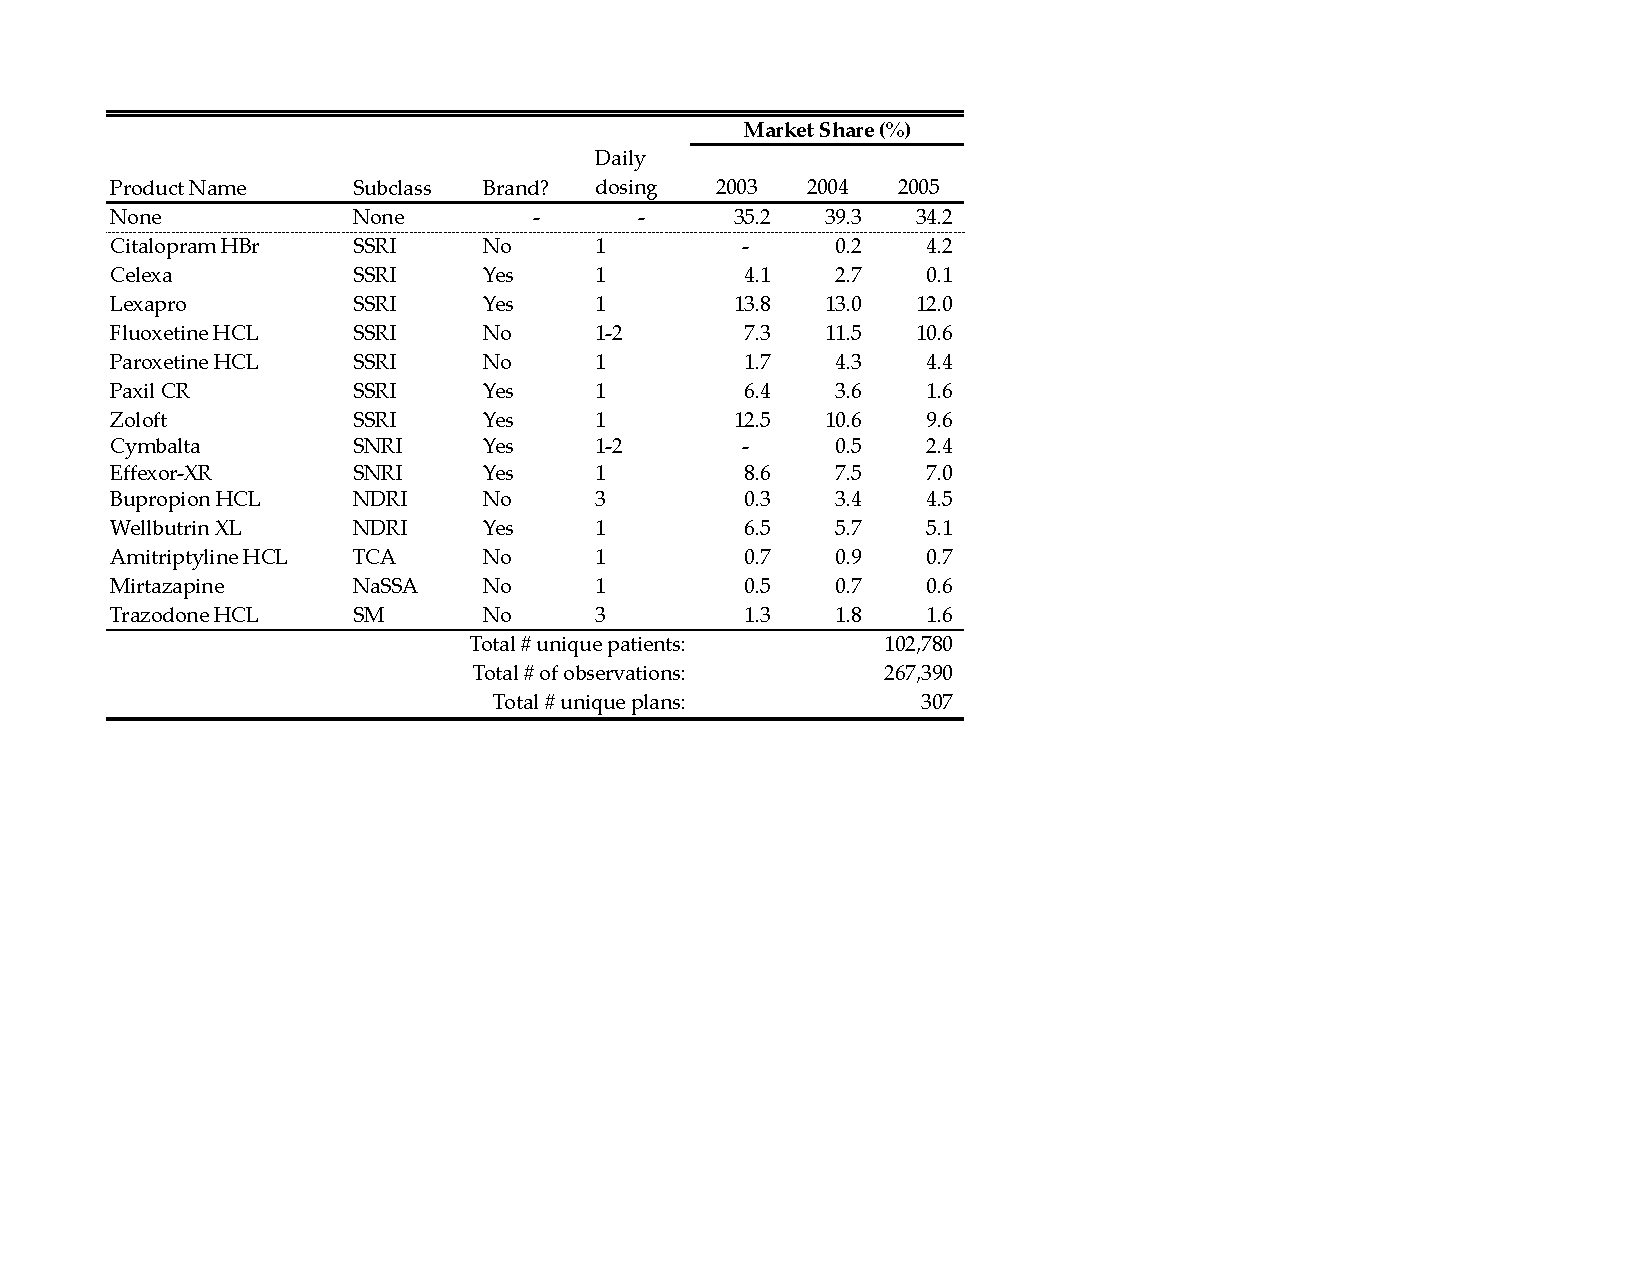
\includegraphics[width=0.9\linewidth]{./resources/slide_shares.pdf}
\end{center}
\end{frame}


\begin{frame}[plain]

\begin{figure}[h!]
\centering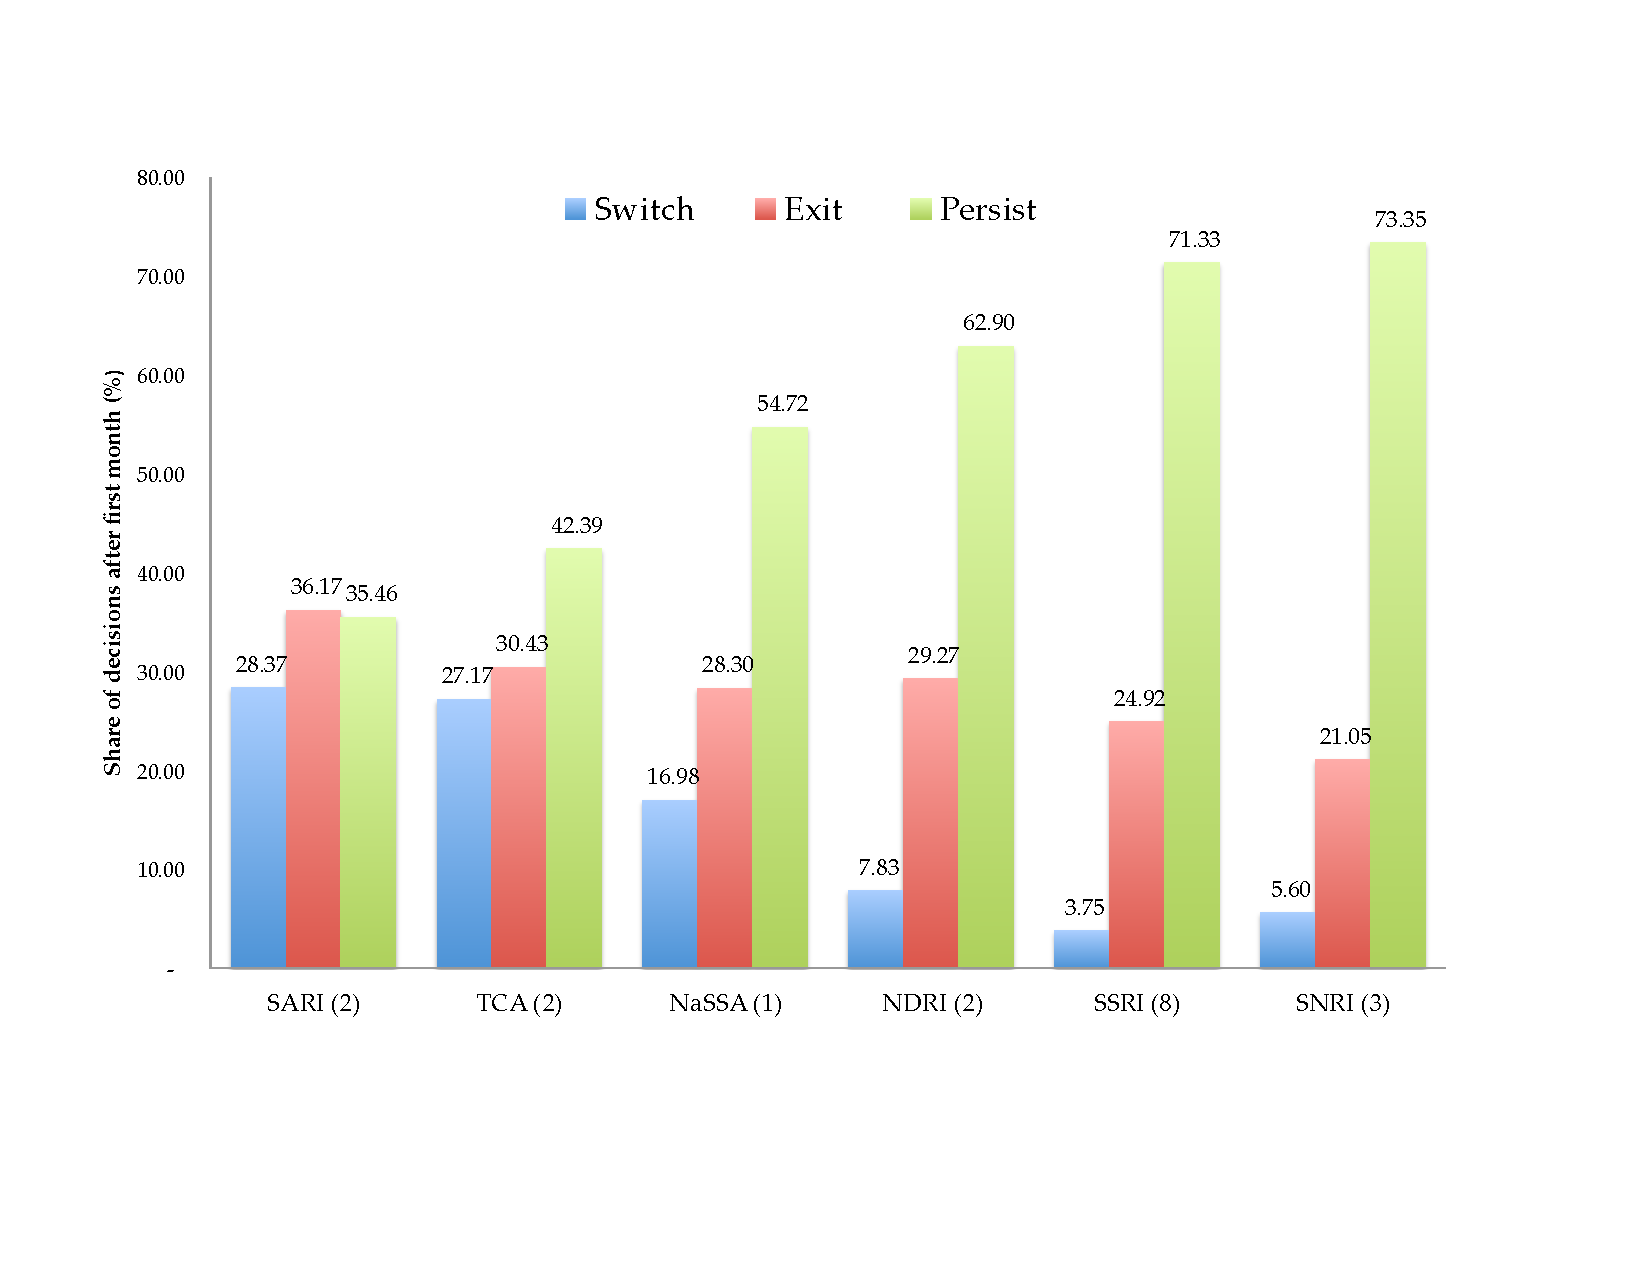
\includegraphics[width=1\linewidth]{./resources/switch_chart.pdf}
\end{figure}

Switch/Quit/Persist across Classes after First Month
\end{frame}

%--------------------------------------------------------------------------------

\begin{frame}
\frametitle{Timing of Switches}

\begin{figure}[h!]
\centering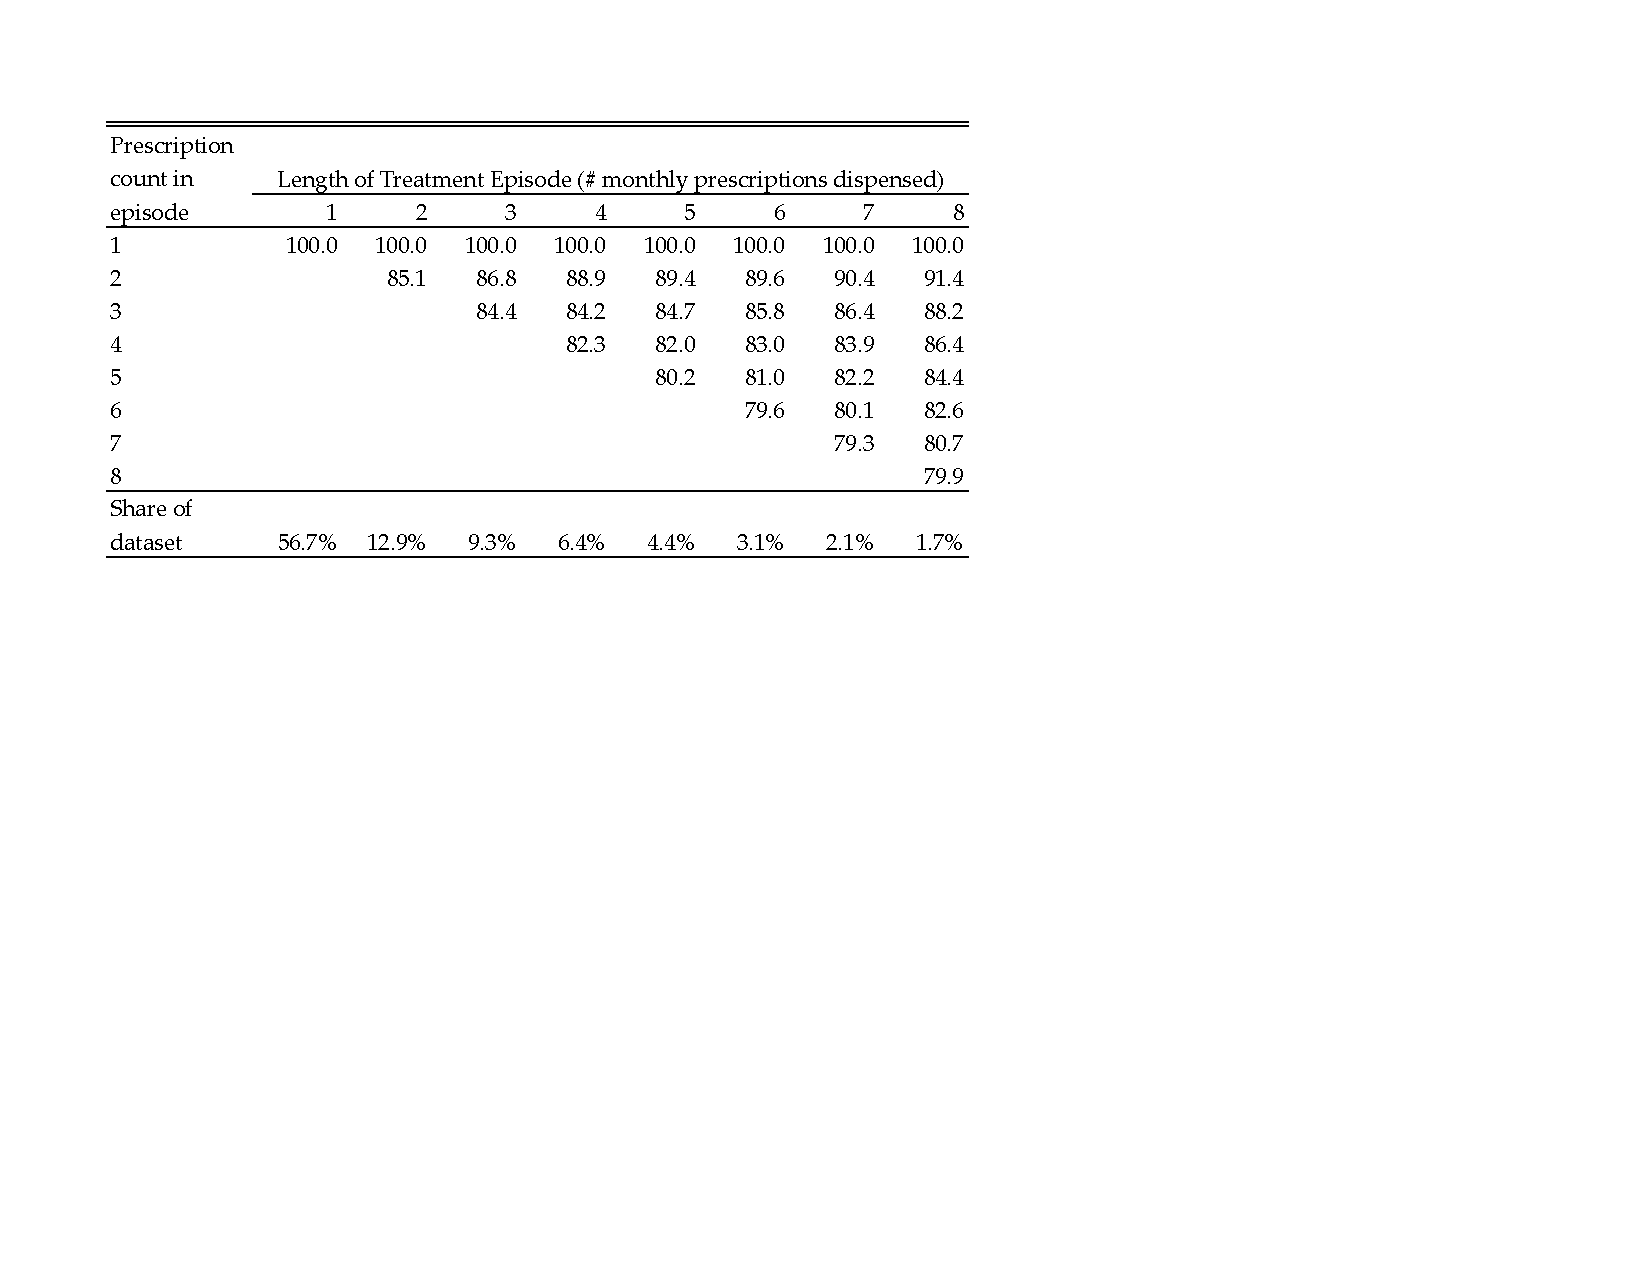
\includegraphics[width=1\linewidth]{./resources/table3_slide.pdf}
\end{figure}
\end{frame}


\begin{frame}
\frametitle{Hazard of switching}

\begin{itemize}
\item Interpret as probability of finding a drug ``ineffective"

\item Condition on patient costs, doses/day, rate of side effects, patient
diagnosis

\item Find range of predicted prob of effectiveness
\end{itemize}

\begin{figure}[h!]
\centering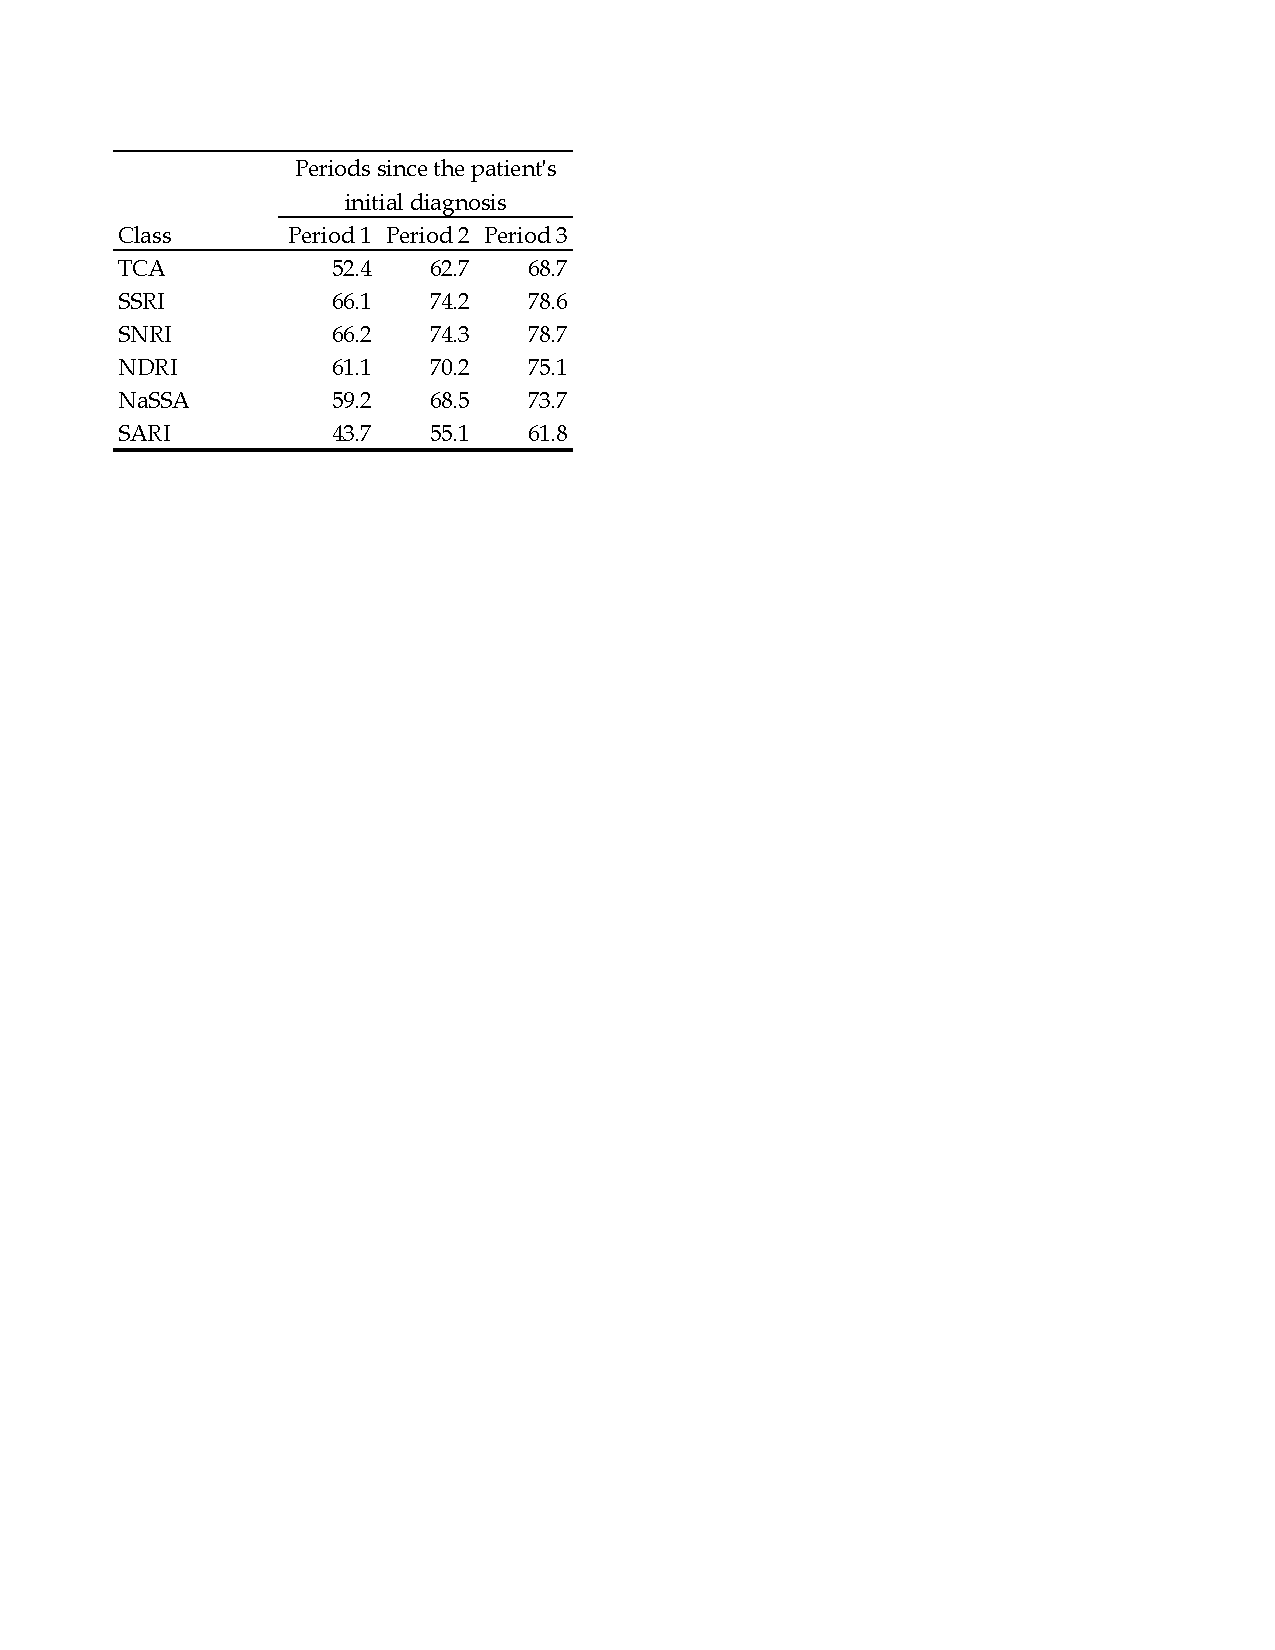
\includegraphics[width=.5\linewidth]{./resources/prob_effective.pdf}
\end{figure}
\end{frame}

\section{Learning Model}

%--------------------------------------------------------------------------------

\begin{frame}
\frametitle{Learning Model}

\textbf{Goal}:

Estimate parameters of the agent's learning process using the timing and
identity of observed switch/persist decisions

\textbf{Requires}:

Predicted choice probabilities to match to observed choices

\begin{itemize}
\item (1) Discrete outcomes

\item (2) Patient and physician priors

\item (3) Updating process

\item (4) Decision rule

\begin{itemize}
\item myopic vs. forward-looking

\item independent vs. correlated choices
\end{itemize}
\end{itemize}
\end{frame}

\begin{frame}
\frametitle{(1) Discrete outcomes}

\begin{itemize}
\item Patient and physician ($i$) observe a discrete outcome, $Y_{ijt}$,
under treatment $j$ at time $t$

\item ``Outcome" includes efficacy, price, side effects, ease of use, ... 
\pause

\item $Y_{ijt}$ drawn from a Bernoulli distribution

\item Probability of a successful outcome equals $p_{j}$:

\[
Y_{ijt}\backsim p_{j}^{k}(1-p_{j})^{1-k},k\in \{0,1\}
\]
where $k=1$ if drug $j$ proves effective in period $t$
\end{itemize}
\end{frame}

%--------------------------------------------------------------------------------

\begin{frame}
\frametitle{(1) Discrete outcomes (continued)}

Prior on $p_{j}$

\begin{itemize}
\item Beta distribution with parameters $(a_{j,0},b_{j,0})$

\item Mean and variance of Beta distribution: 
\begin{eqnarray*}
\mu _{j,0} &=&\frac{a_{j,0}}{a_{j,0}+b_{j,0}}  \label{mean_parm} \\
v_{j,0} &=&\frac{a_{j,0}b_{j,0}}{(a_{j,0}+b_{j,0})^{2}(a_{j,0}+b_{j,0}+1)}
\end{eqnarray*}
where $a_{j,0}>0$ and $b_{j,0}>0$.
\end{itemize}
\end{frame}

%--------------------------------------------------------------------------------

\begin{frame}
\frametitle{(2) Updating process}

After $t$ trials of treatment $j$:

\begin{itemize}
\item add to $a_{j,0}$ the number of successes observed

\item add to $b_{j,0}$ the number of failures observed
\end{itemize}

Why?

\begin{itemize}
\item Beta is conjugate prior for Bernoulli likelihood. So, posterior
distribution of $p_{j}$ is Beta.
\end{itemize}

Caveat

\begin{itemize}
\item In the application, successes and failures not observed; I integrate
over the discrete number of possible realizations.
\end{itemize}
\end{frame}

\begin{frame}
\frametitle{(3) Decision Rule: Options}
\small
(1) `Bayesian Myopic' at $(T+1)$ after updating using $\widehat{Y}_{ij}$: 
\[
\max_{j\in 1,...,J}E(p_{i,j,T+1}|a_{0},b_{0},\widehat{Y}_{ij}) +
\varepsilon_{ijt}=\mu _{j,T+1} + \varepsilon_{ijt} 
\]

\begin{itemize}
\item Experience on $j$ for periods $t=1,...,T$ in vector $\widehat{Y}_{ij}$

\item Choose what to consume at $T+1$

\item $\varepsilon_{ijt}$ represents idiosyncratic tastes for $j$ at $t$
\end{itemize}
\end{frame}

%--------------------------------------------------------------------------------

\begin{frame}
\frametitle{(3) Decision Rule: Options}
\small

(2) `Forward-Looking' at $(T+1)$ after updating using $\widehat{Y}_{ij}$:%
\[
\max_{j\in 1,...,J}\mu _{j,T+1} + h(V(p_{i,j,T+1}|a_{0},b_{0},\widehat{Y}%
_{ij})) + \varepsilon_{ijt} 
\]
\end{frame}

%--------------------------------------------------------------------------------

\begin{frame}
\frametitle{(3) Decision Rule: Forward-Looking Problem}
\small

The physician and patient choose a sequence of drugs to maximize the
expected discounted sum of outcomes, $Y_{t}$: 
\begin{equation}
\int ...\int E_{p_{1},...,p_{J}}\left( \sum_{t=1}^{\infty }\delta
^{t-1}Y_{t}\right) d\Pi ^{(1)}(p_{1})\cdots d\Pi ^{(J)}(p_{J})
\label{seq_prob}
\end{equation}

\begin{itemize}
\item $\delta$ is given and $p=(p_{1},...,p_{J})$ is the unknown vector of
probabilities that a drug $j\in{1,...,J}$ is effective.

\item the agent forms independent priors, $\Pi $, on the elements of $p$

\item The state variables include the number of successes and failures under
each choice
\end{itemize}
\end{frame}

%--------------------------------------------------------------------------------

\begin{frame}[label=ALTERNATIVES]

\frametitle{(3) Decision Rule: Forward-Looking Solutions}
\small

Solutions:

\begin{itemize}
\item Dynamic Programming, via Rust (1987) and Hotz and Miller (1993)

\item Keane and Wolpin (1984), simulation and interpolation

\item Gittins' (1979) index rule: Break $J$-dimensional problem into $J$
continue-quit decisions, one for each choice

\begin{itemize}
\item Inner maximization: solve 1-dim optimal stopping problem for each $j$.
Save discounted expected value, the ``index"

\item Outer maximization: choose $j$ with the maximal index value
\end{itemize}
\end{itemize}
\end{frame}

\begin{frame}[label=DYNAM]

\frametitle{(3) Decision Rule: Forward-Looking Solutions}
\small

Requirements for Gittins' Index:

\begin{enumerate}
\item the decision-maker selects only one option at $t$

\item options not chosen remain in their initial state

\item each option is independent

\item options not selected do not contribute to the individual's outcome
\end{enumerate}

\hyperlink{GITTINS}{\beamerbutton{More on Gittins}}
\end{frame}

%--------------------------------------------------------------------------------

\begin{frame}
\frametitle{(3) Decision Rule: Forward-Looking Solutions}
\small

My approach (computable via forward induction):

\begin{itemize}
\item Use index rule, treating each drug compound choice as independent

\begin{itemize}
\item unobservables not correlated across drug choices
\end{itemize}

\item Use index rule with explicit nesting structure

\begin{itemize}
\item use drug classes as nests, within which choices may be correlated

\item unobservables not correlated across drug classes
\end{itemize}
\end{itemize}
\end{frame}

%--------------------------------------------------------------------------------

\begin{frame}[label=RULE]

\frametitle{(3) Decision Rule: Index Rule form}
\small

Apply forward induction rule 
\[
G(\Pi _{t}^{(j)})=\mu _{j,t}+\sqrt{v_{j,t}}*\left[\psi \left( \frac{v_{j,t}}{%
h(\delta)\ast \sigma ^{2}(\mu _{j,t})}\right)\right]
\]

\begin{itemize}
\item $(\mu _{j,t},v_{j,t})$, are the mean and variance of the posterior
beta distribution for $p_{j}$, the probability that drug $j$ is effective.

\item $\psi(.)$ represents the closed-form numerical approximation to the
boundary of the one-dimensional optimal stopping problem for each drug
(Chang and Lai (1987))
\end{itemize}
\end{frame}

%--------------------------------------------------------------------------------

\begin{frame}
\frametitle{(3) Decision Rule: Index Rule form}

\[
G(\Pi _{t}^{(j)})=\mu _{j,t}+\sqrt{v_{j,t}}*\left[\psi \left( \frac{v_{j,t}}{%
h(\delta)\ast \sigma ^{2}(\mu _{j,t})}\right)\right]
\]

\begin{eqnarray*}
\mu _{j,t} &=&\frac{a_{j,t}}{a_{j,t}+b_{j,t}} \\
v_{j,t} &=&\frac{a_{j,t}b_{j,t}}{(a_{j,t}+b_{j,t})^{2}(a_{j,t}+b_{j,t}+1)} \\
\sigma ^{2}(\mu _{j,t}) &=&\mu _{j,t}\ast (1-\mu _{j,t})
\end{eqnarray*}

Experimentation incentive diminishes when:

\begin{itemize}
\item $\delta $ is small, $h(\delta)$ is large

\item when past experience diminishes $v_{j,t}$

\item when $\sigma ^{2}(\mu _{j,t})$ is large
\end{itemize}
\end{frame}

%--------------------------------------------------------------------------------

\begin{frame}
\frametitle{(3) Decision Rule: Index Rule with Correlation} %
\framesubtitle{via Pandey et al. (2007)}

\begin{figure}[h!]
\centering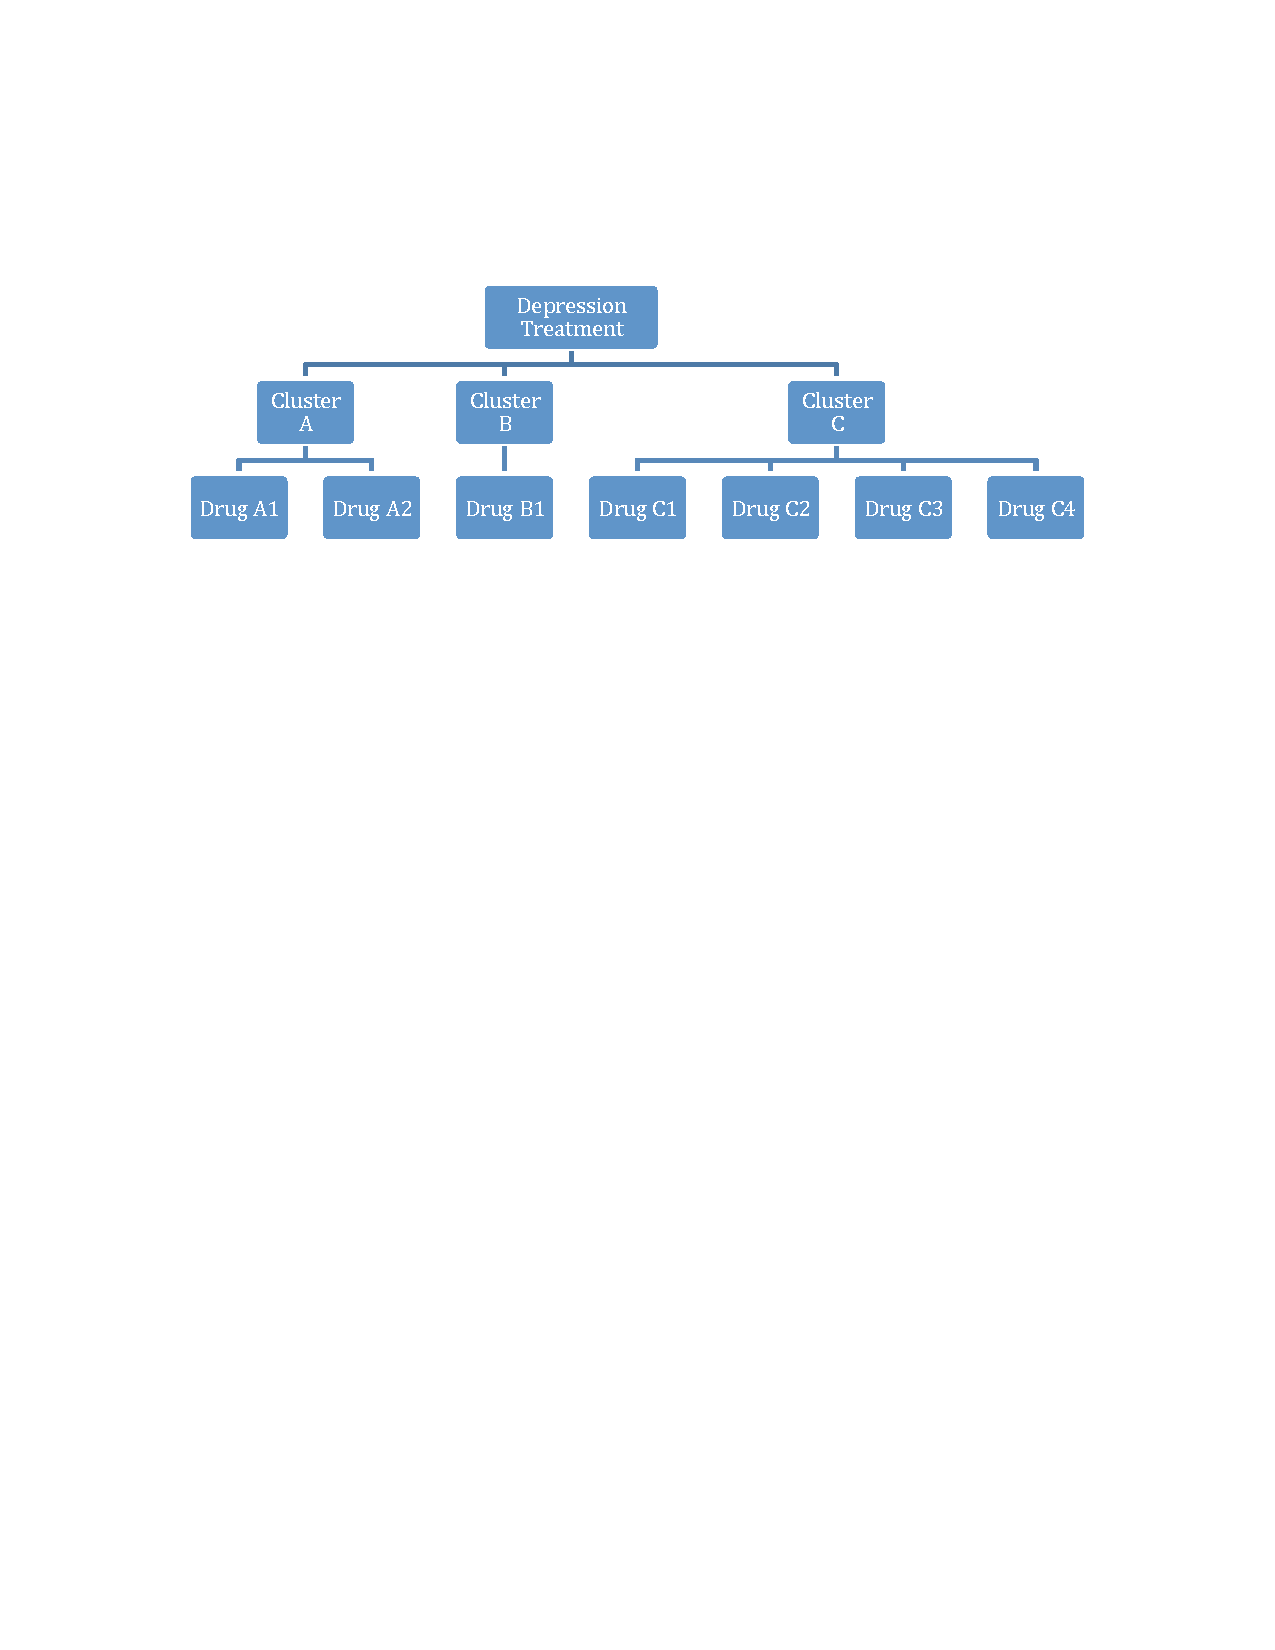
\includegraphics[width=1\linewidth]{./resources/drug_hierarchy.pdf}
\end{figure}

\begin{itemize}
\item Cluster by drug class

\item Sum outcomes over all trials of drugs within the class 
\begin{eqnarray*}
a_{c,t} &=&\sum_{j}1\{j\in c\} \ast a_{j,t} \\
b_{c,t} &=&\sum_{j}1\{j\in c\} \ast b_{j,t}
\end{eqnarray*}
\end{itemize}
\end{frame}

%--------------------------------------------------------------------------------

\begin{frame}
\frametitle{(3) Decision Rule: Index Rule with Correlation}

\begin{itemize}
\item Index rule for the class 
\[
G(\Pi _{t}^{(c)})=\mu _{c,t}+\sqrt{v_{c,t}}*\left[\psi \left( \frac{v_{c,t}}{%
h(\delta)\ast \sigma ^{2}(\mu _{c,t})}\right)\right]
\]

\item Drug class choice probability 
\[
\text{Prob}_{c,t}=\frac{\exp (G(\Pi _{t}^{(c)}))}{1+\sum_{s=1}^{C-1}\exp
(G(\Pi _{t}^{(s)}))}
\]

\item Drug compound choice probability 
\begin{eqnarray*}
\text{Prob}_{j\in c,t} &=&\text{Prob}_{c,t}\text{(Prob}_{j,t}|\text{1\{c
chosen\})} \\
&=&\text{Prob}_{c,t}\ast \frac{\exp (G(\Pi _{t}^{(j)}))}{\sum_{k\in c}\exp
(G(\Pi _{t}^{(k)}))}
\end{eqnarray*}
\end{itemize}
\end{frame}

\section{Estimates and Fit}

%--------------------------------------------------------------------------------

\begin{frame}
\frametitle{Econometric Model}

\begin{itemize}
\item Parameterize $p_{j}$ using beta regression model 
\begin{eqnarray*}  \label{mu_logit}
p_{j}|X_{ij} &\backsim &Beta(a_{0},b_{0}) \\
\mu(X_{ij};\gamma_{1}) &=& \frac{a_{o}}{a_{0}+b_{0}} = \frac{\exp
(X_{ij}\gamma_{1} )}{1+\exp(X_{ij}\gamma_{1} )} \\
\phi(\gamma_{2}) &=& a_{0}+b_{0}=\exp(\gamma_{2})
\end{eqnarray*}

where $\mu$ is prior mean, $\phi$ is the prior precision of $p_{j}$

\item The prior variance of $p_{j}$ is: 
\begin{eqnarray*}
V(p_{j}|X_{ij})&=&\frac{\mu(1-\mu)}{1+\phi}
\end{eqnarray*}

\item For a fixed $\mu$, the larger the value of $\phi$, the smaller the
variance in $p_{j}$.
\end{itemize}
\end{frame}

%--------------------------------------------------------------------------------

\begin{frame}[plain]

\begin{figure}[h!]
\centering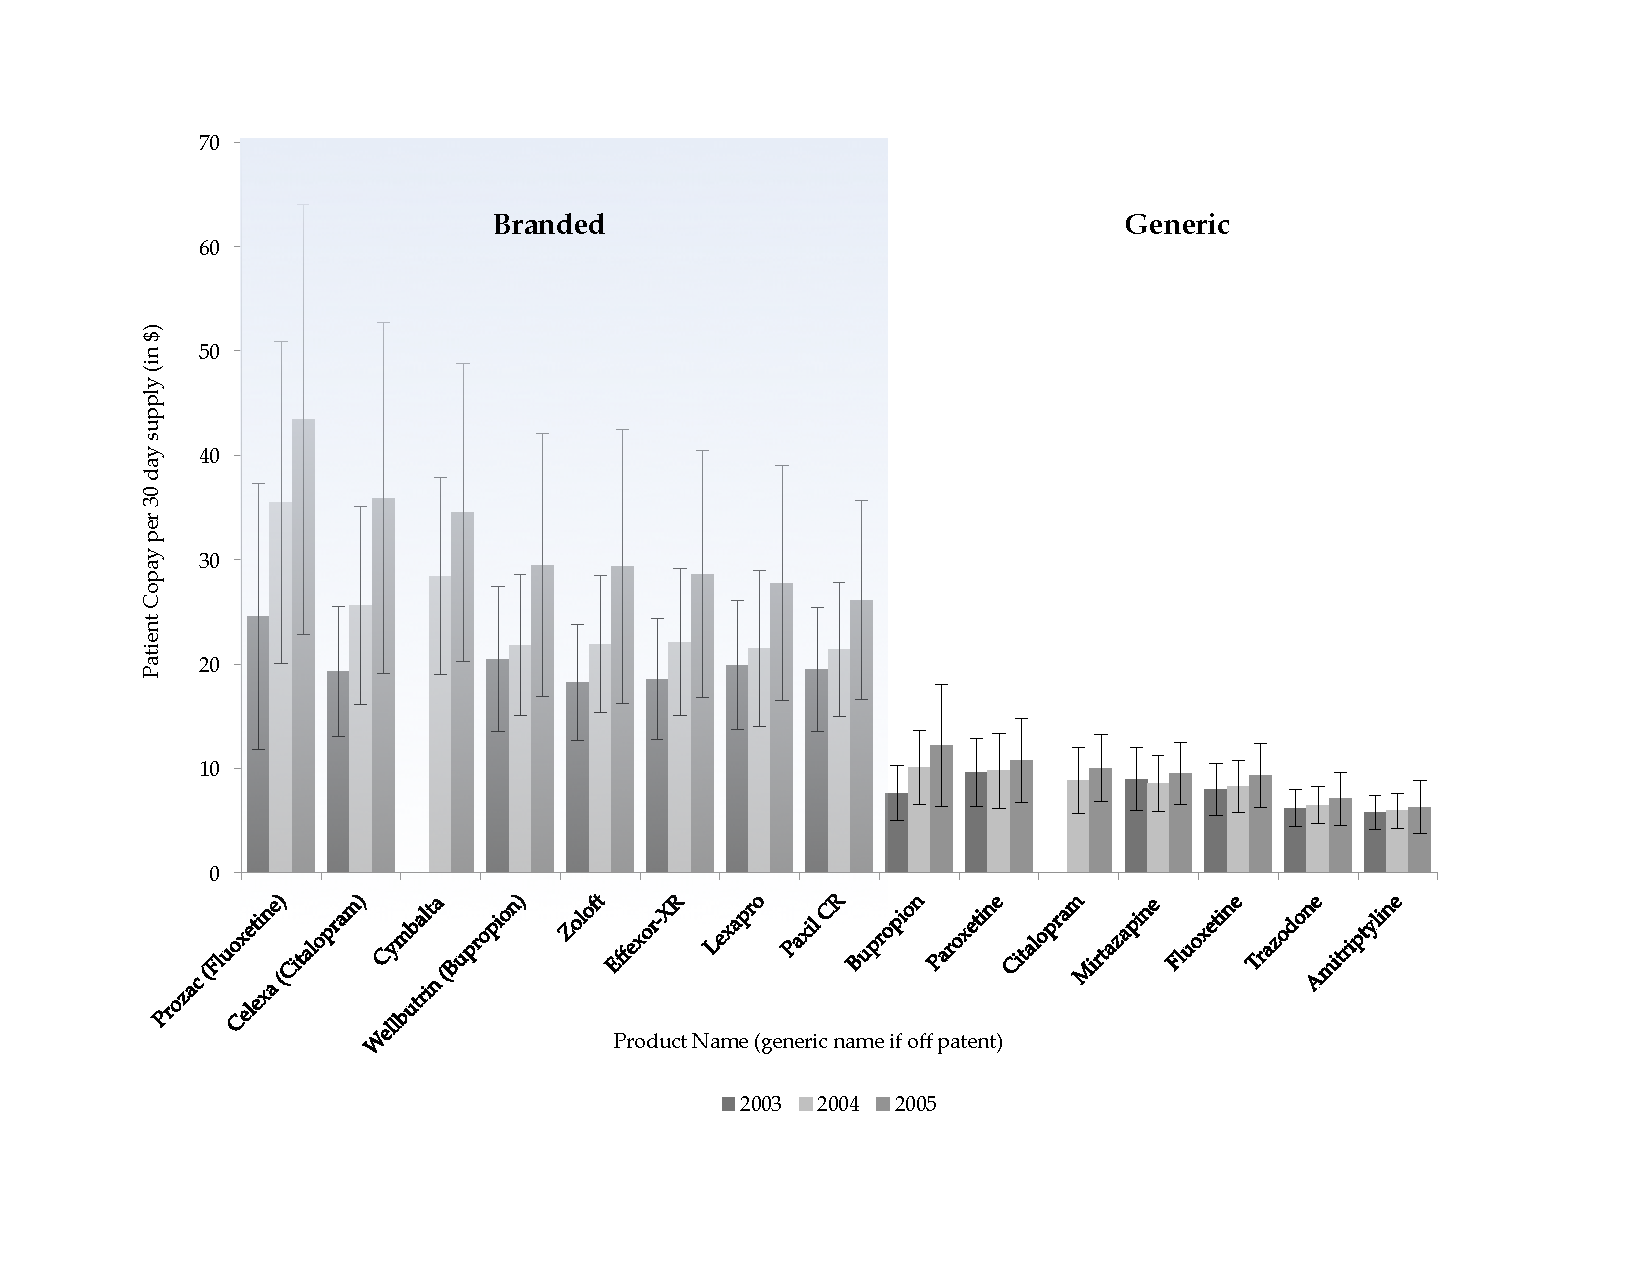
\includegraphics[width=0.7\linewidth]{./resources/fig1.pdf}
\end{figure}

Figure 1: Patient Copayments by Product and Year (standard deviation across
insurance plans shown)
\end{frame}

%--------------------------------------------------------------------------------

\begin{frame}[plain]

\begin{figure}[h!]
\centering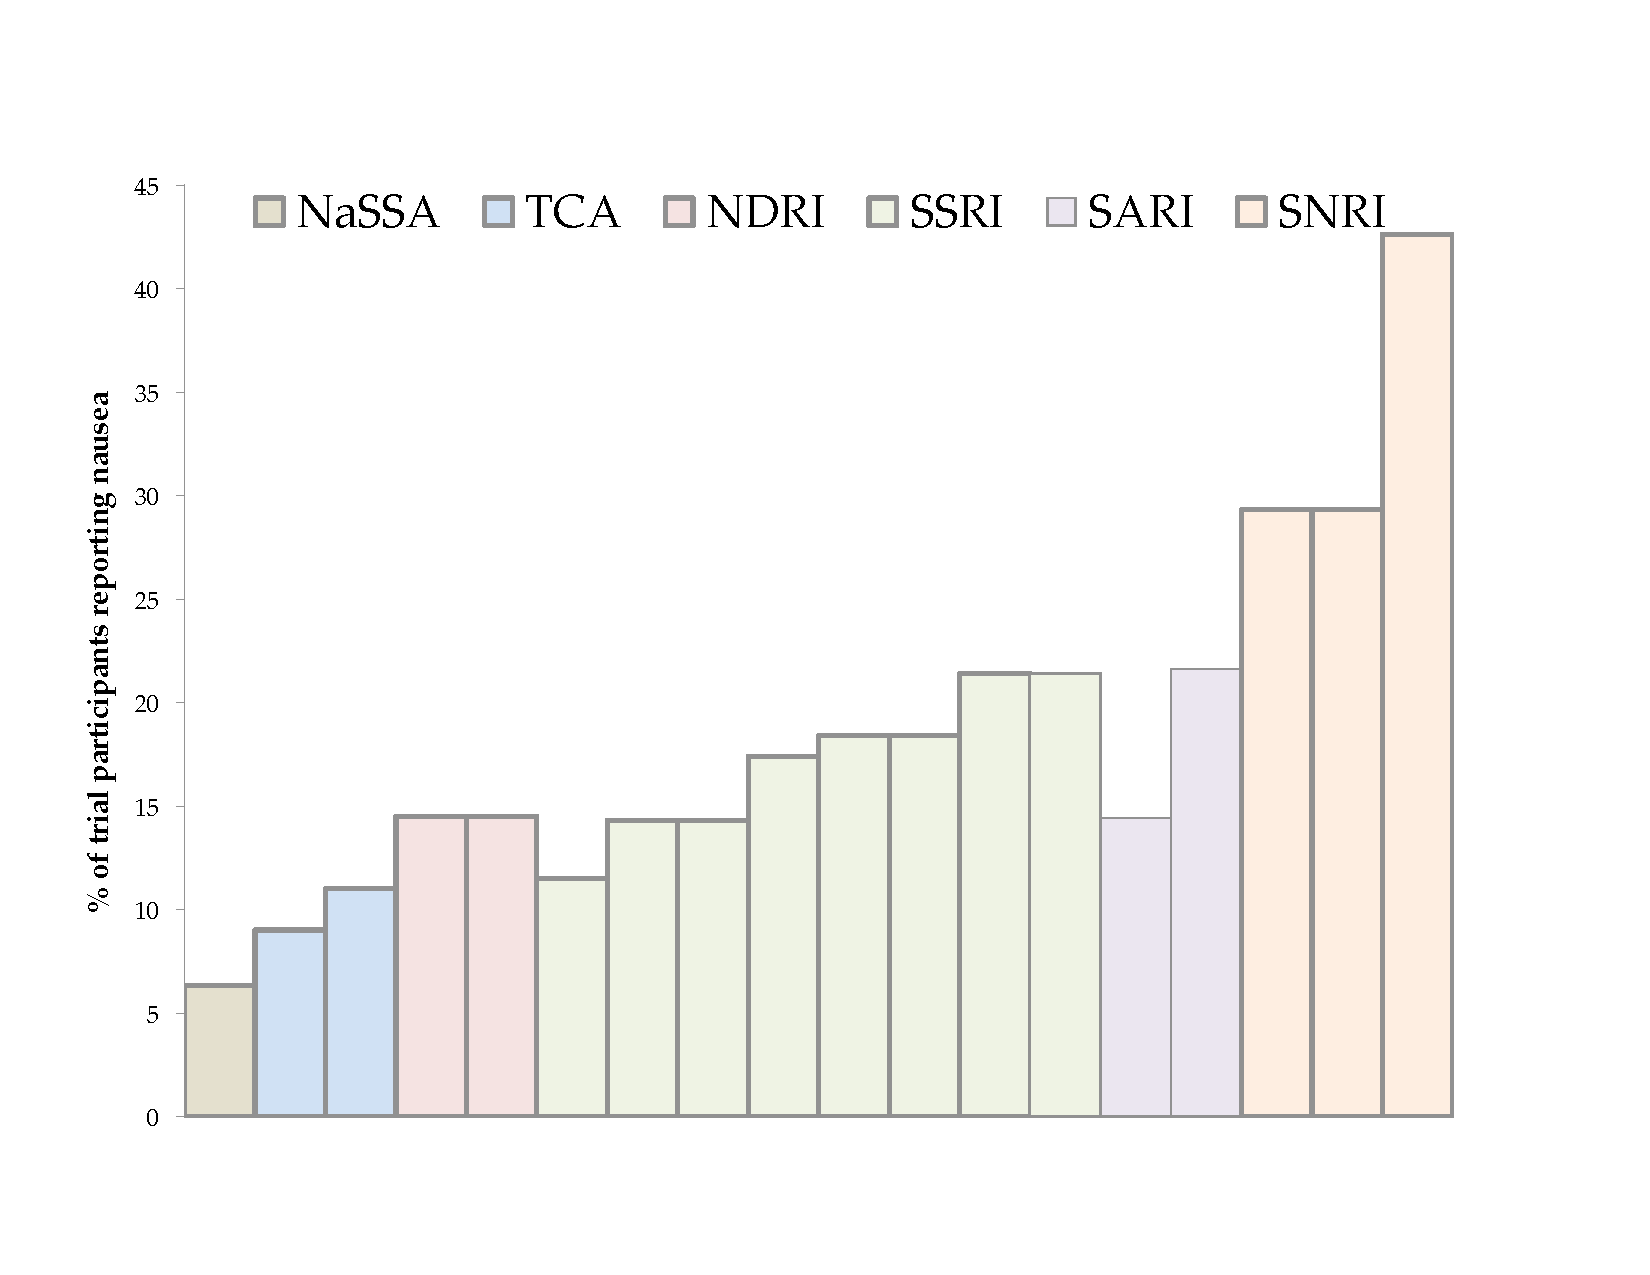
\includegraphics[width=0.7\linewidth]{./resources/nausea_fig.pdf}
\end{figure}

Figure 2: Nausea Side Effects in Clinical Trials
\end{frame}

%--------------------------------------------------------------------------------

\begin{frame}
\frametitle{Identification}

Goal: recover $\gamma=(\gamma_{1},\gamma_{2})$, in the mean and precision of 
$p_{j}$

\begin{enumerate}
\item Identity of choice throughout the sequence of treatments

\begin{itemize}
\item Identifies expected mean outcome under available choices following
standard arguments
\end{itemize}

\item Information on drug characteristics from clinical trial data, external
sources

\item Timing of observed switches

\begin{itemize}
\item Identifies precision of the agents' priors

\item Slowing switching, condition on $\mu$, higher uncertainty in agents'
priors

\item Errors assumed idiosyncratic
\end{itemize}
\end{enumerate}
\end{frame}

%--------------------------------------------------------------------------------

\begin{frame}
\frametitle{Results, via maximum likelihood}

\begin{figure}[h!]
\centering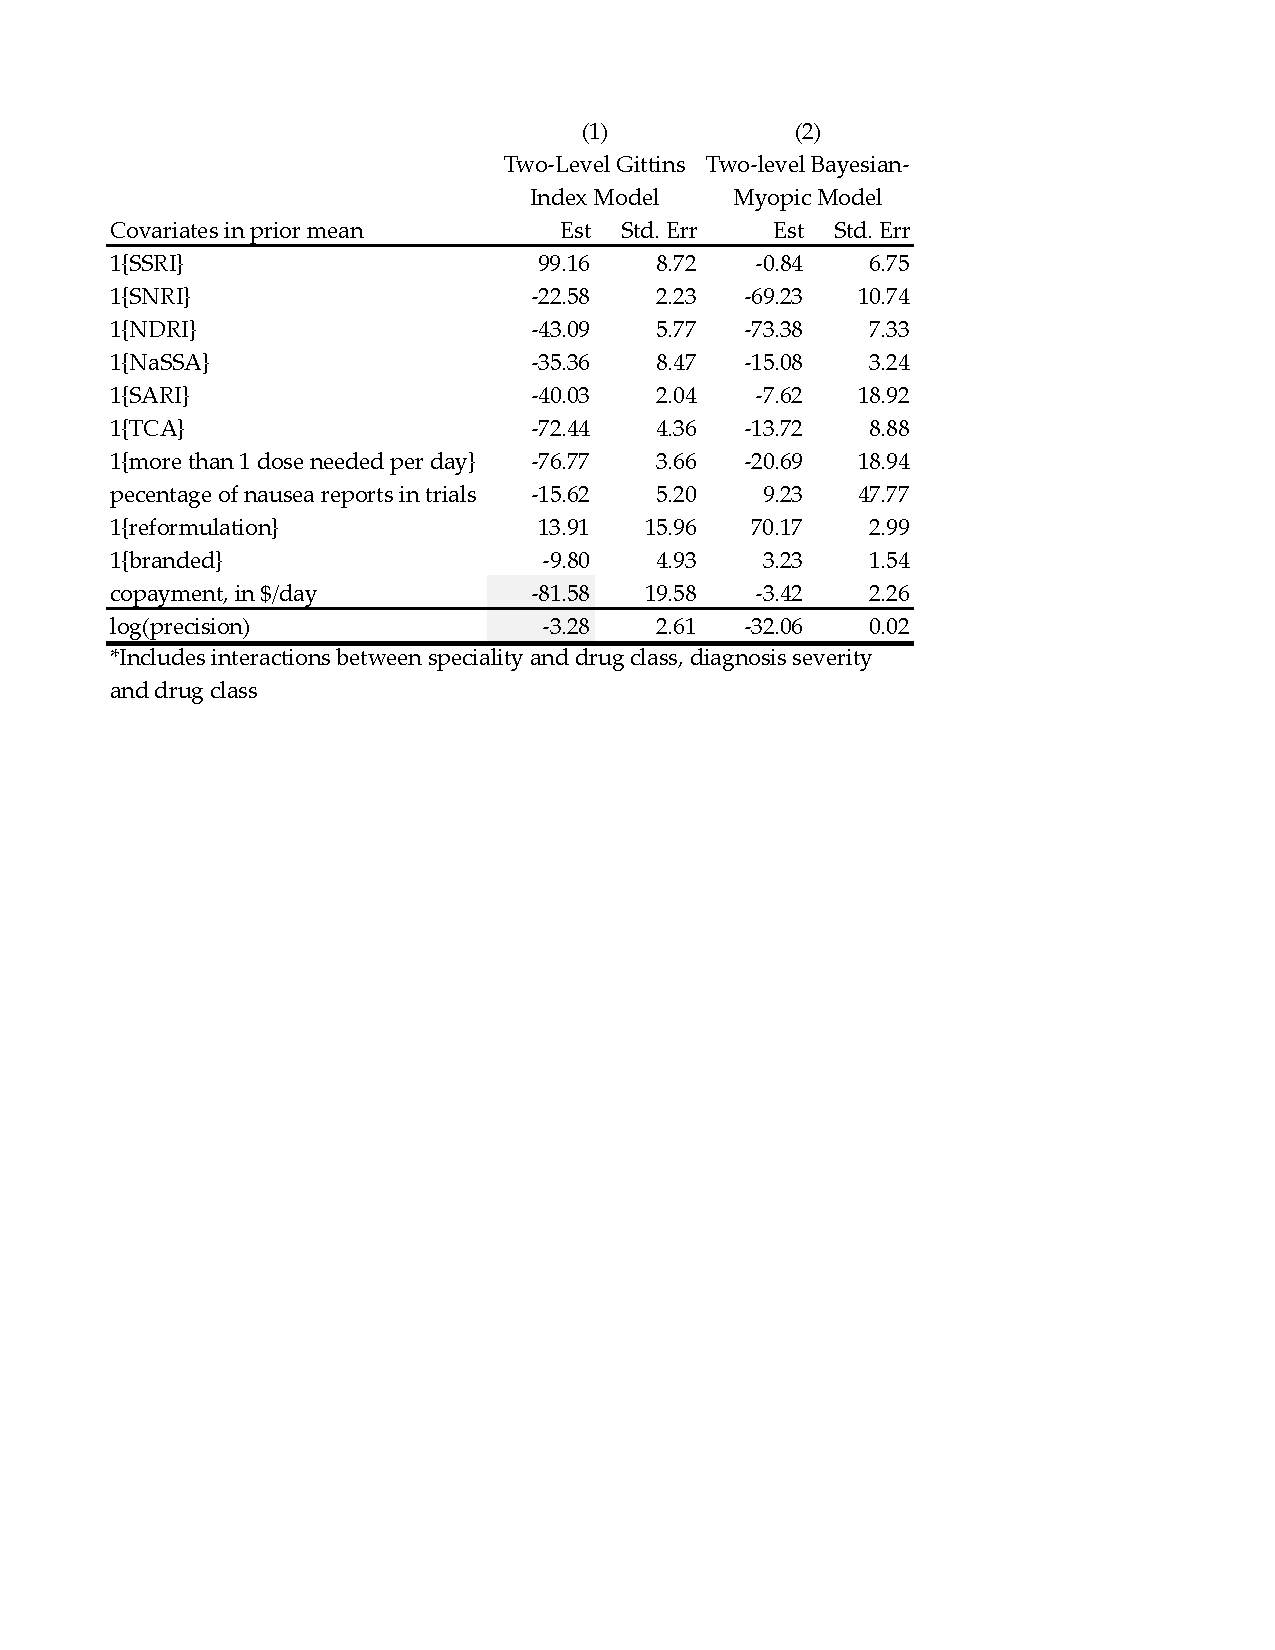
\includegraphics[width=0.8\linewidth]{./resources/est_table.pdf}
\end{figure}

\hyperlink{ESTIMATION}{\beamerbutton{Estimation Details}}
\end{frame}

%--------------------------------------------------------------------------------

\begin{frame}
\frametitle{Fit - Adherence Rate}

\begin{figure}[h!]
\centering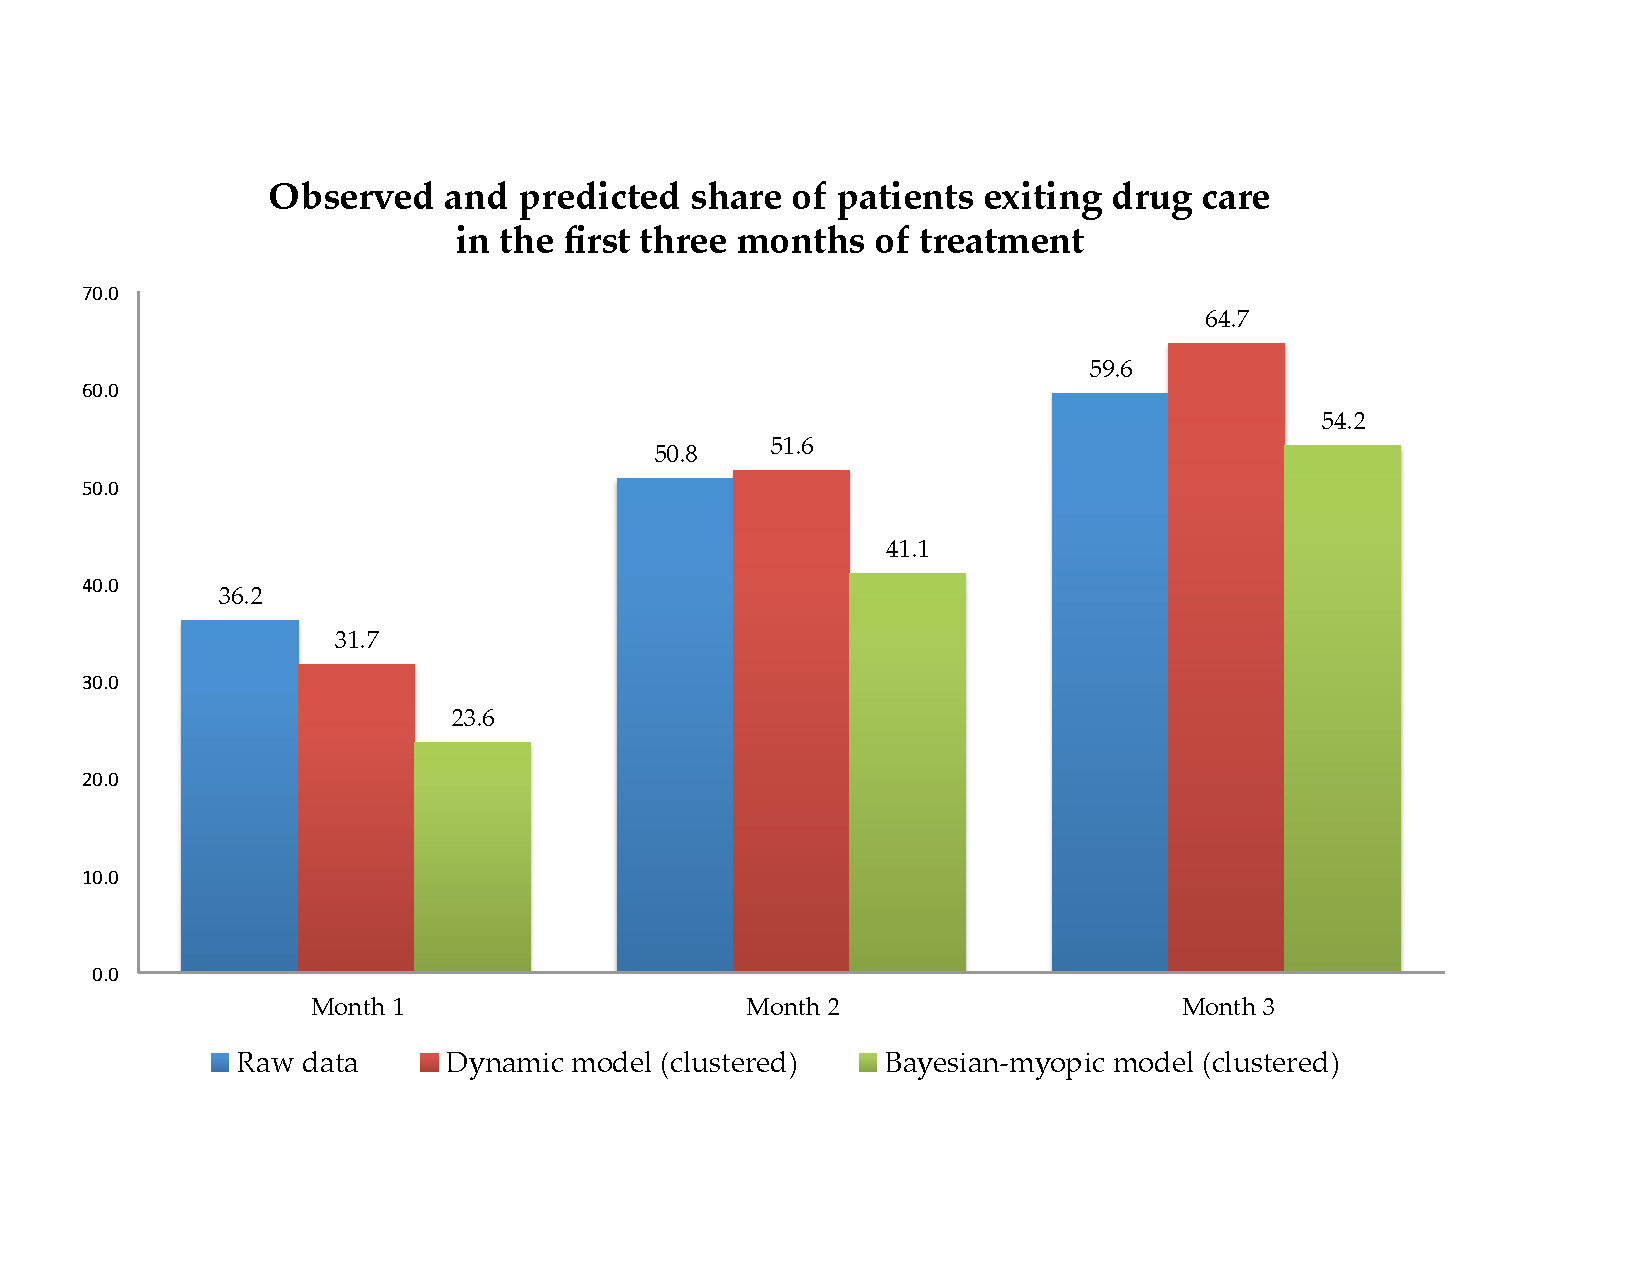
\includegraphics[width=1\linewidth]{./resources/fit_adherence_chart.pdf}
\end{figure}
\end{frame}

%--------------------------------------------------------------------------------

\begin{frame}
\frametitle{Fit: Predicted Choices by Individual}

\begin{figure}[h!]
\centering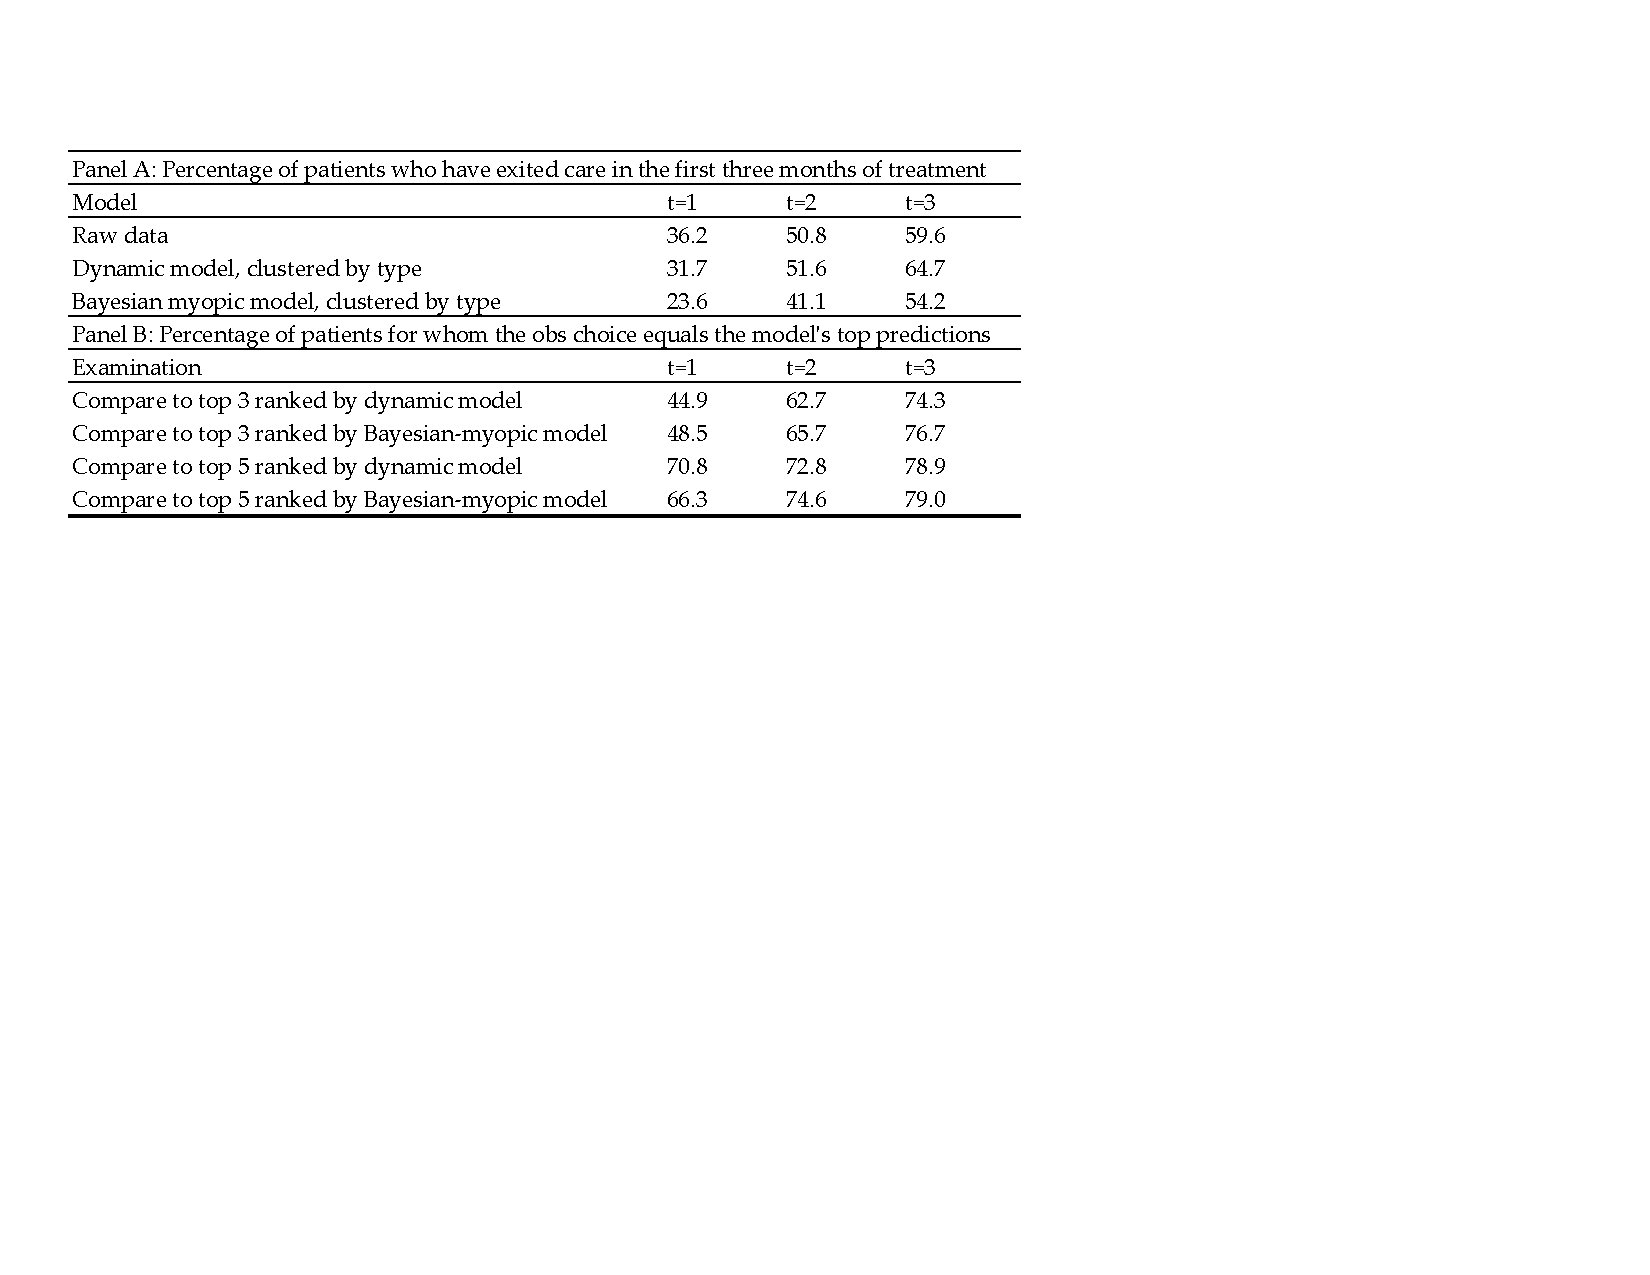
\includegraphics[width=1\linewidth]{./resources/fit_table.pdf}
\end{figure}

\begin{itemize}
\item Kullback-Leibler Information Criterion: 11.95

\item At the 95\% critical value, the data favors the two-level dynamic
model over the one-level model.
\end{itemize}
\end{frame}

\section{Counterfactuals}

%--------------------------------------------------------------------------------

\begin{frame}
\frametitle{Counterfactuals: Shares in the First Month}

\begin{figure}[h!]
\centering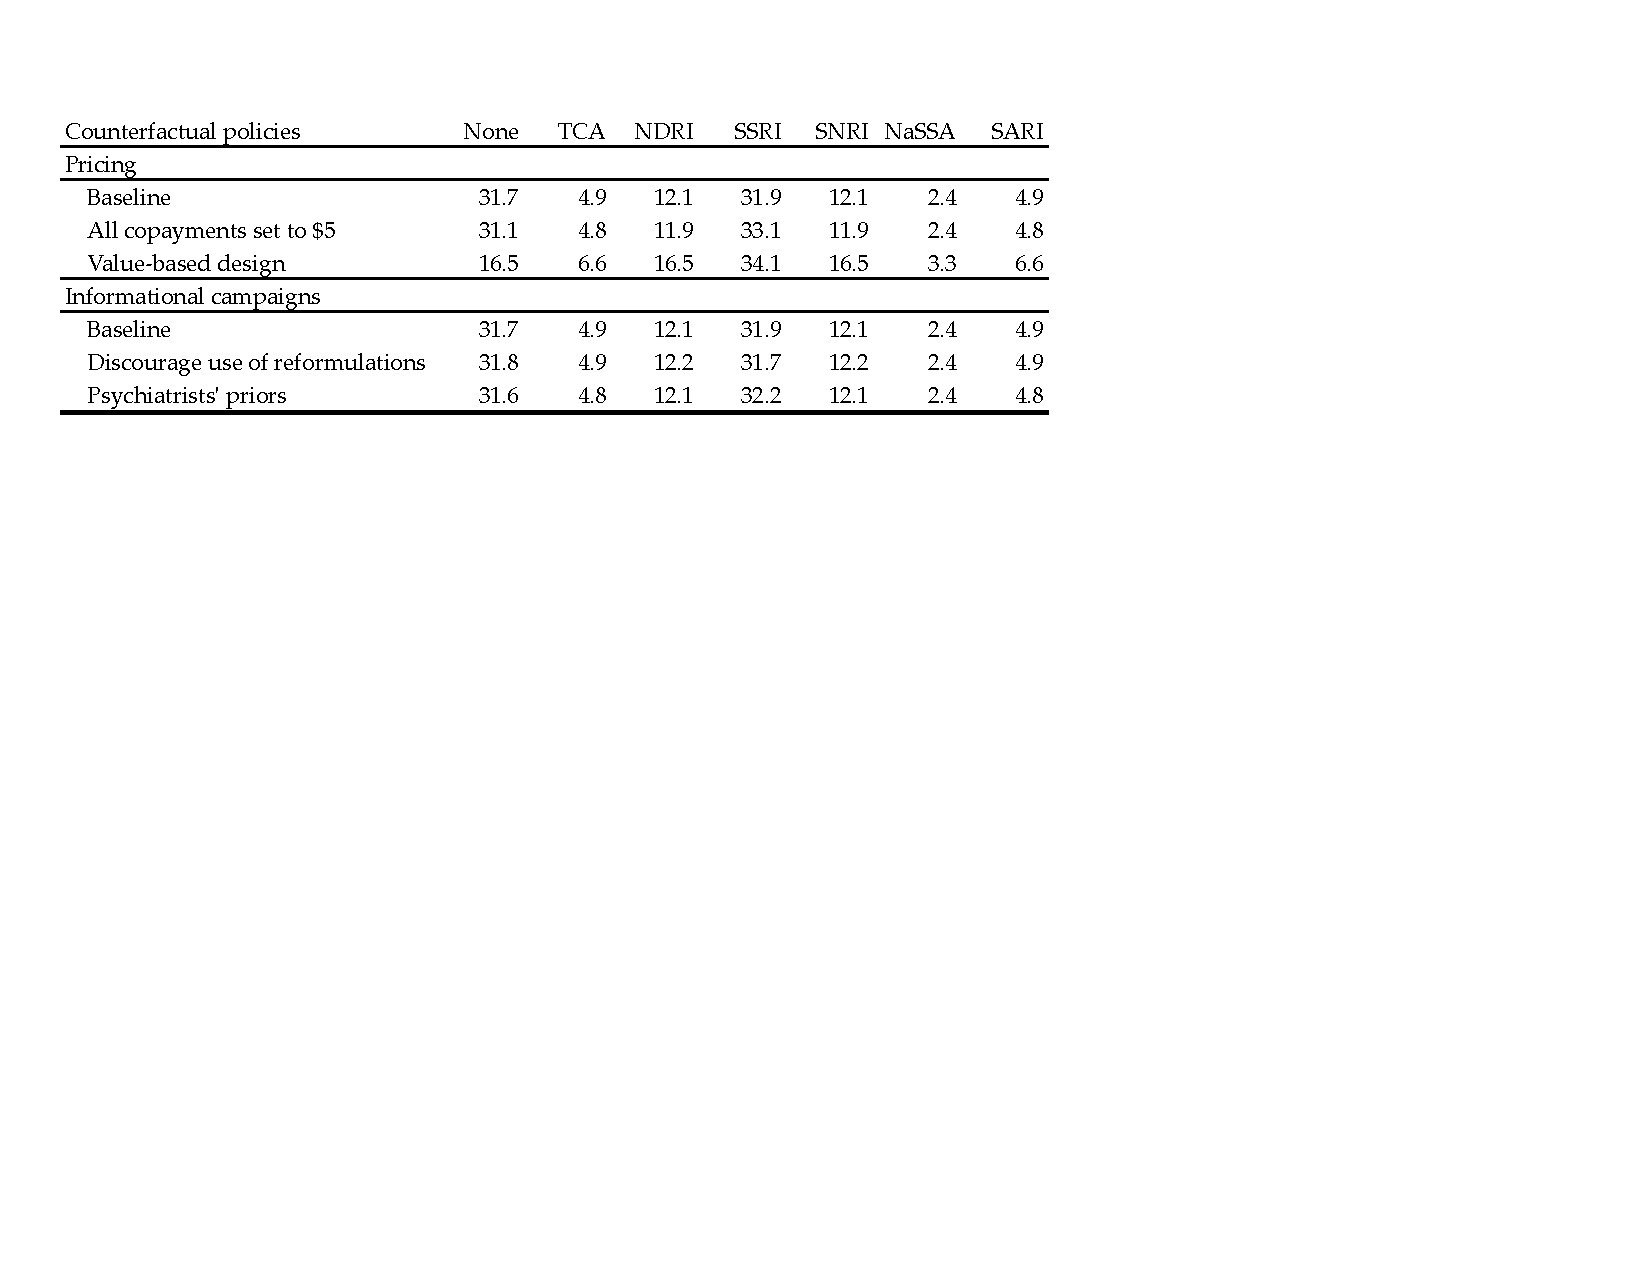
\includegraphics[width=1.0\linewidth]{./resources/ctfl_slide.pdf}
\end{figure}
\end{frame}

%--------------------------------------------------------------------------------

\begin{frame}
\frametitle{Counterfactuals: Calculating dollar value of health}

\begin{itemize}
\item Berndt et al. (2002) provides recovery rates of first 16 weeks of care
(via expert panel)

\begin{itemize}
\item e.g. Patient on SSRI for $>30$ days has $.28$ rate of recovery, $.60$
rate of partial recovery
\end{itemize}

\item Convert each individual's choice to an expected number of weeks with
full/partial symptoms over first 16 weeks%
\[
\text{%
\begin{tabular}{|l|l|l|}
\hline
Treatment & Full (wks) & Partial (wks) \\ \hline
No Drug Care & $11.9$ & $2.8$ \\ \hline
$\text{SSRI, }\leq \text{30 days}$ & $10.3$ & $3.9$ \\ \hline
$\text{SSRI, }> \text{30 days}$ & $7.3$ & $5.9$ \\ \hline\hline
\end{tabular}%
} 
\]

\item Lave et al. (1998): disutility from full depression, -.41

\item Covert utility change (in weeks) to dollars using \$100,000 value of
year of life (Cutler (2004))
\end{itemize}
\end{frame}

%--------------------------------------------------------------------------------

\begin{frame}[label=WELFARE]

\frametitle{Counterfactuals: Cost and health comparison}

\begin{figure}[h!]
\centering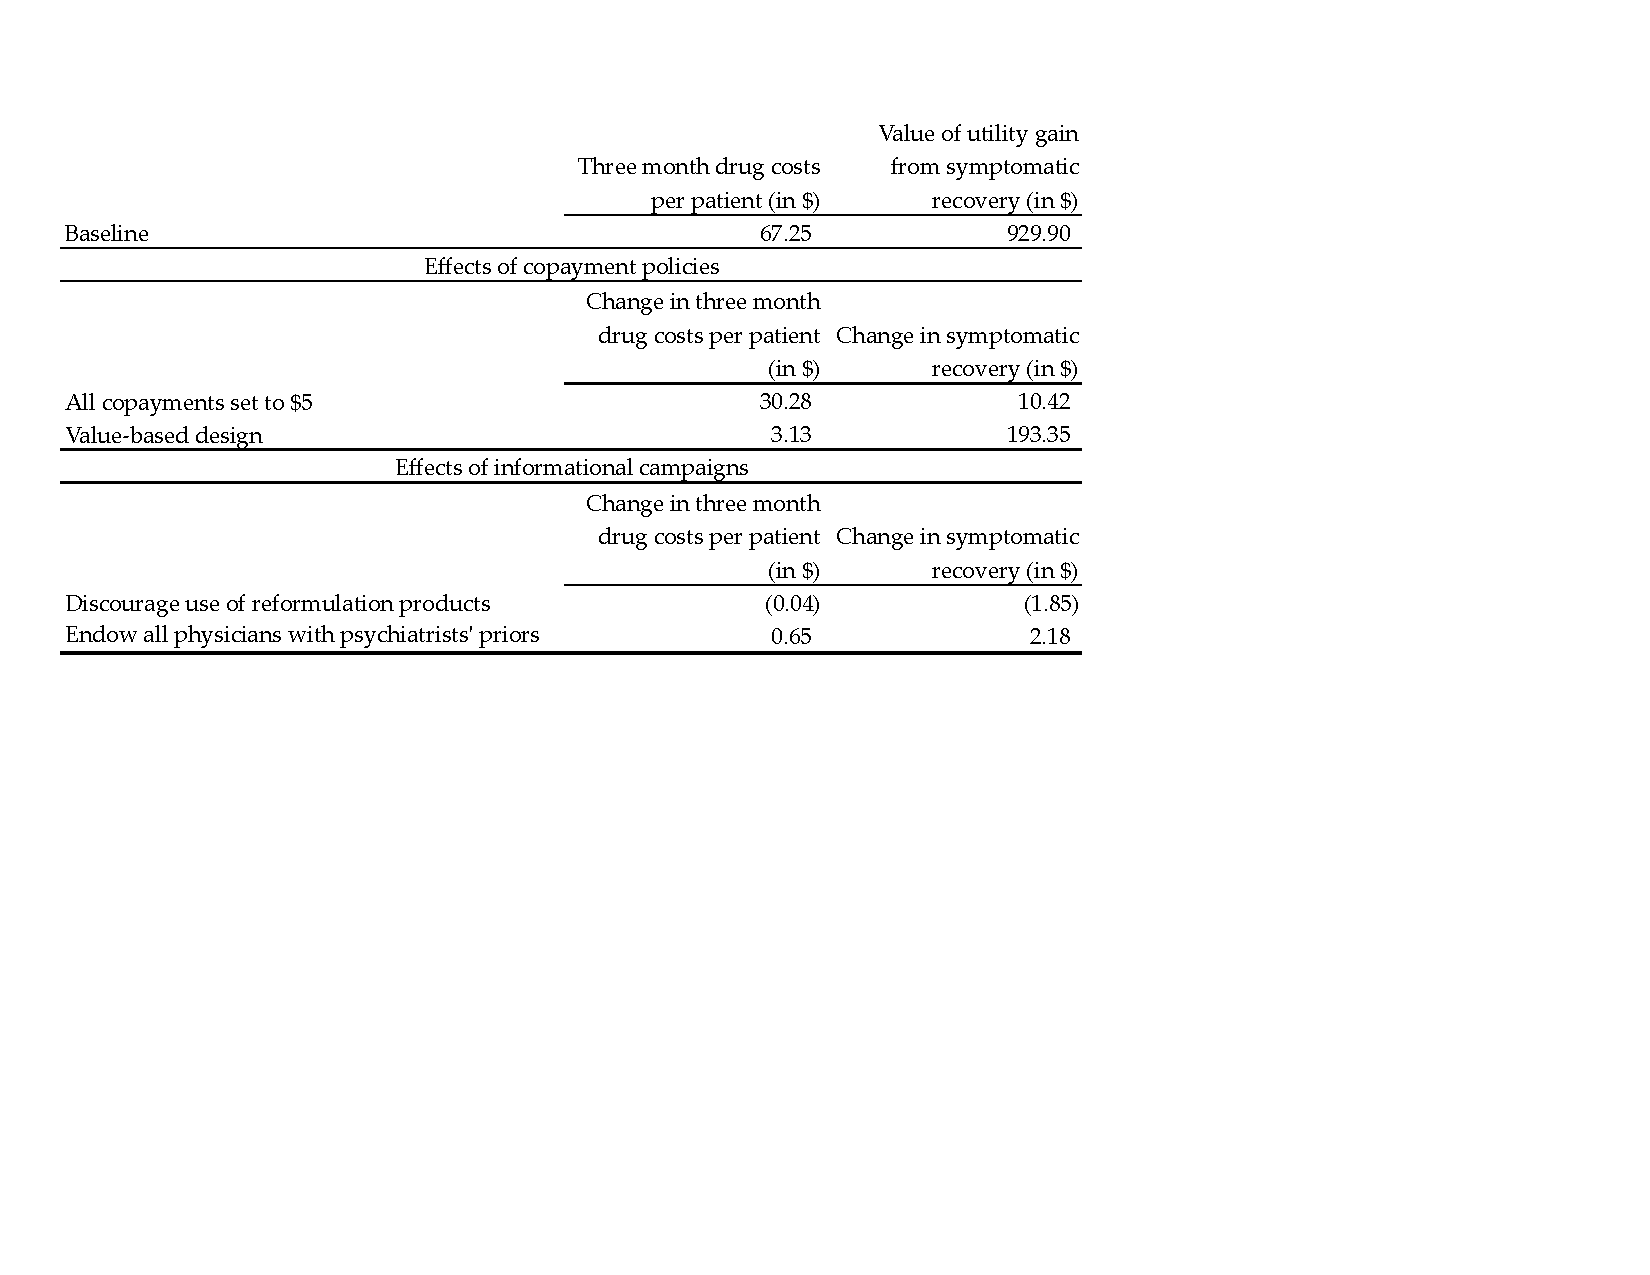
\includegraphics[width=1\linewidth]{./resources/welfare_table.pdf}
\end{figure}
\end{frame}

%--------------------------------------------------------------------------------

\begin{frame}[plain]

\frametitle{Counterfactuals: New Protocol}

\begin{figure}[h!]
\centering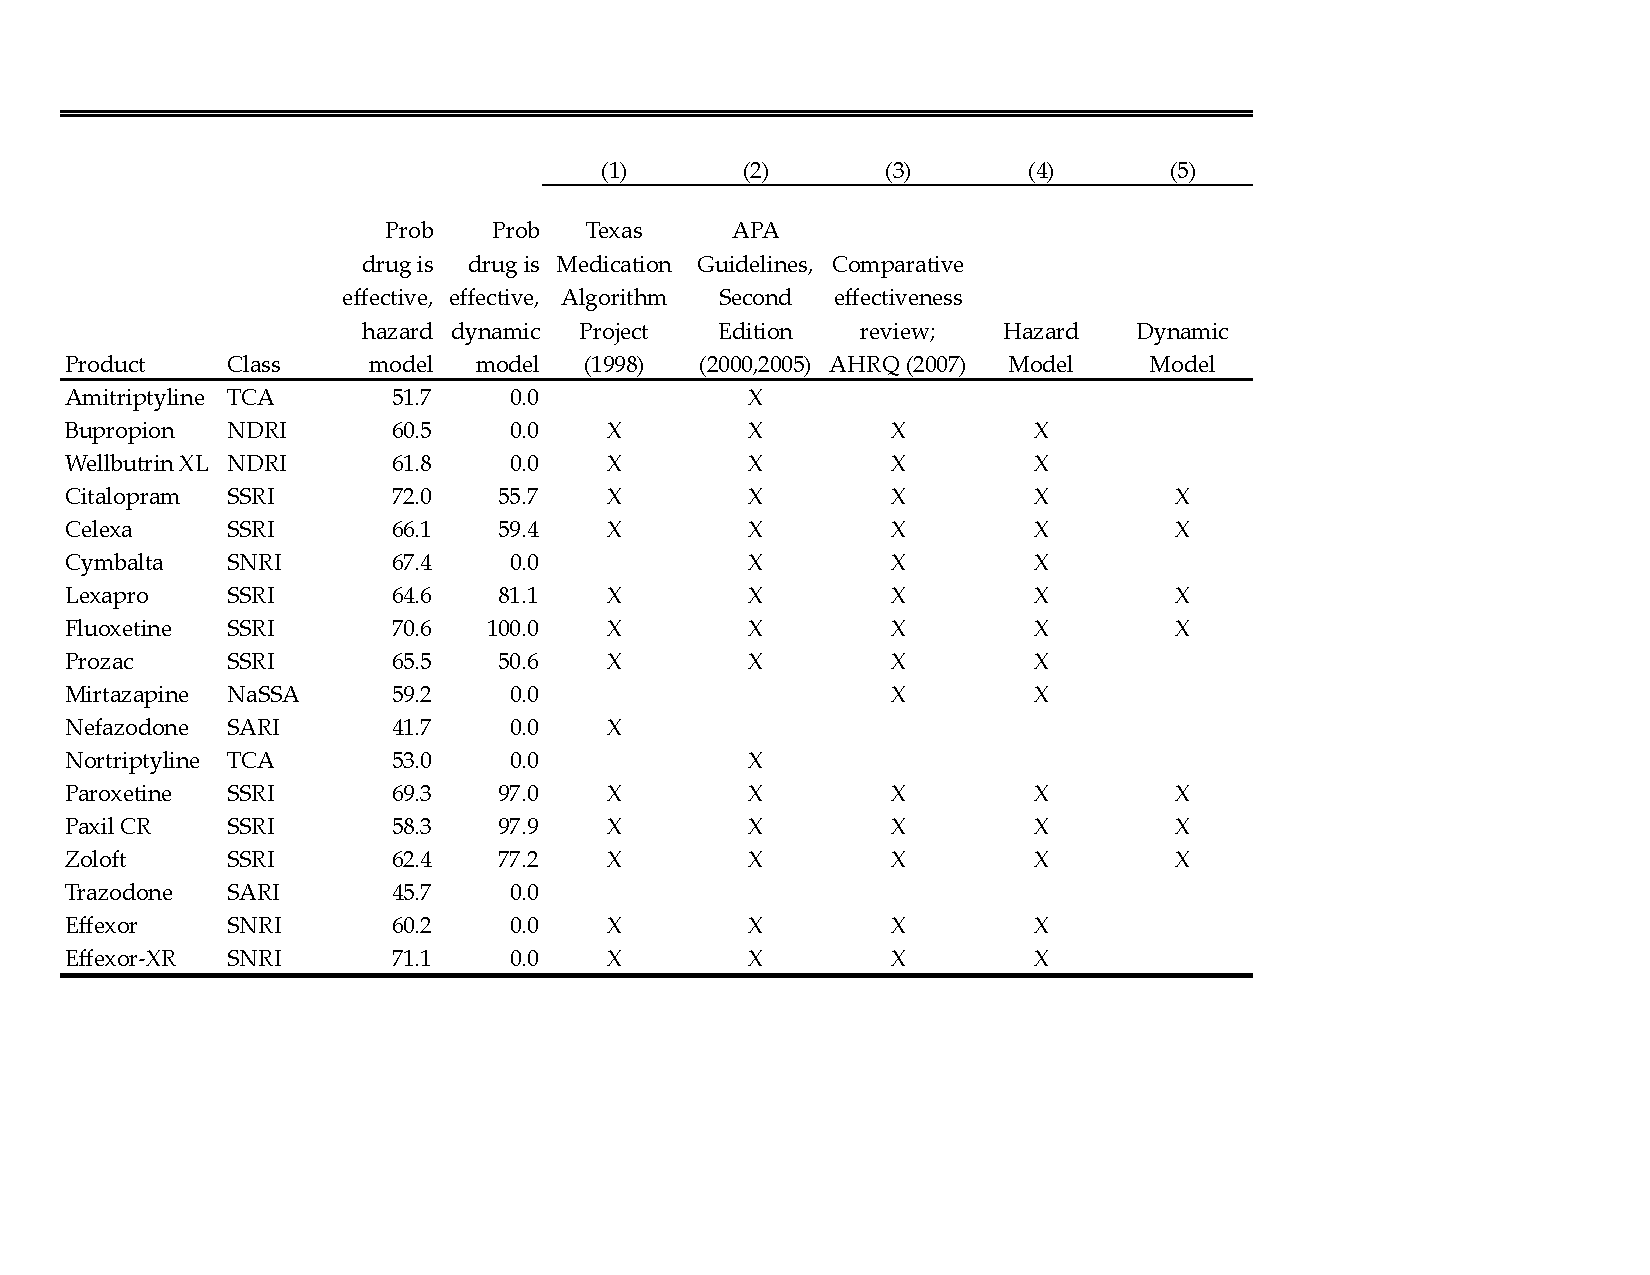
\includegraphics[width=1.\linewidth]{./resources/protocol.pdf}
\end{figure}
\end{frame}

%--------------------------------------------------------------------------------

\begin{frame}[label=ESTIMATION]

\frametitle{Estimation: Likelihood form}

When we assume independent products, the likelihood for individual $i$ in
period $t$ is:%
\begin{multline*}
\prod_{j=1}^{J}E_{\varepsilon _{i1t},...,\varepsilon _{iJt}}(1\{G_{ijt}(\Pi
_{t}^{(j)})+\varepsilon_{ijt}>G_{ikt}(\Pi _{t}^{(k)})+\varepsilon_{ikt}\text{
for all }k\neq j\}^{d_{ijt}}) \\
=\prod_{j=1}^{J}\left( \frac{\exp (G_{ijt}(X_{ij},\widehat{Y}%
_{i,j,t-1};\gamma ))}{1+\sum_{k}\exp (G_{ikt}(X_{ik},\widehat{Y}%
_{i,k,t-1};\gamma )}\right) ^{d_{ijt}}
\end{multline*}

\begin{itemize}
\item $G_{ijt}$ is the index rule

\item $d_{ijt}=1$ if $i$ chooses drug $j$ in period $t$

\item $\widehat{Y}_{i,l,t-1}$ is a vector of realized outcomes under
treatments $l=1,...,J$ during the previous $(t-1)$ periods

\item $\varepsilon _{ijt}$ follow an extreme value distribution
\end{itemize}
\end{frame}

%--------------------------------------------------------------------------------

\begin{frame}
\frametitle{Estimation: Likelihood form}

\begin{itemize}
\item $(\widehat{Y}_{i,1,t-1},...,\widehat{Y}_{i,J,t-1})$ are latent

\item Sum over the possible sequences of outcomes, weighting by the
probability of observing those sequences
\end{itemize}

\[
\sum_{s}\omega_{i,s}\prod_{j=1}^{J}\left( \frac{\exp (G_{ijt}(X_{ij},%
\widehat{Y}^{s}_{i,j,t-1};\gamma ))}{1+\sum_{k}\exp (G_{ikt}(X_{ik},\widehat{%
Y}^{s}_{i,k,t-1};\gamma )}\right) ^{d_{ijt}}
\]

\begin{itemize}
\item $\omega_{i,s}$ is the probability of observing one of $s\in S$
possible sequences; follows a discrete binomial distribution

\item $\widehat{Y}^{s}_{i,j,t-1}$ represents discrete counts of successes
and failures realized over $(t-1)$ periods.

\item Under rational expectations, the parameters that underlie $\omega_{i,s}
$ equal the parameters of the agents' priors.
\end{itemize}

\hyperlink{RESULTS}{\beamerbutton{Return to Results}}
\end{frame}

%--------------------------------------------------------------------------------

\begin{frame}
\frametitle{Estimation: Likelihood form} \framesubtitle{With dependency
across the drugs via clusters}

{\footnotesize 
\[
\sum_{s}\omega_{i,s}\prod_{c=1}^{C}\left[\left( \frac{\exp (G_{ict}(\Pi
_{t}^{(c),s}))}{1+\sum_{m}^{C-1}\exp (G_{imt}(\Pi _{t}^{(m),s})}\right)
^{d_{ict}}\prod_{j\in c}^{J_{c}}\left( \frac{\exp (G_{ijt}(\Pi _{t}^{(j),s}))%
}{\sum_{k}^{J_{c}}\exp (G_{ikt}(\Pi _{t}^{(k),s})}\right) ^{d_{ijt}}\right]
\]
}{\normalsize where drug $j$ is a choice contained in class $c$. \bigskip }

\begin{itemize}
\item {\normalsize Calculate the choice probabilities at two levels: }

\begin{enumerate}
\item {\normalsize the probability of a class being chosen }

\item {\normalsize the conditional probability of a drug being chosen,
conditional on the class choice }
\end{enumerate}
\end{itemize}

{\normalsize \hyperlink{RESULTS}{\beamerbutton{Return to Results}} }
\end{frame}

%--------------------------------------------------------------------------------

\begin{frame}[label=GITTINS]

\frametitle{Decision Rule: Index Solution}

\begin{itemize}
\item $X_{k}(t)$ \ - the state variables of the choice problem at $t$
(depends on $\widehat{Y}_{t-1}$)

\item At $t$, the agent chooses $j$ if and only if:%
\[
G_{j}(X_{j}(t))=\max_{k\in \{1,...,J\}}G_{k}(X_{k}(t)) 
\]%
\[
G_{j}(x_{j}(t))=\sup_{\tau \geq t}\left\{ \frac{E_{t}\left[ \sum_{r=t}^{\tau
}\beta ^{r-t}R_{j}(X_{j}(r))|x_{j}(t)\right] }{E_{t}\left[ \sum_{r=t}^{\tau
}\beta ^{r-t}|x_{j}(t)\right] }\right\} 
\]

\item $R_{j}(X_{j}(r))$ - the returns from option $j$ given the state
variables at time $r$
\end{itemize}

\hyperlink{DYNAM}{\beamerbutton{Return to Decision Rule}}
\end{frame}



\end{document}













































